%%%%%%%%%%%%%%%%%%%%%%%%%%%%%%%%%%%%%%%%%%%%%%%%%%%%%%%%%%%%%%%%%%%%%%%%%%%%%%%%%%%%%%%%%%%%%
%% Modelo.tex  (Serve para escrever Monografias - Dissertação - Tese)                      %%
%%                                                                                         %%
%% Idealizado em  06/12/2012 - por:  Emivan Ferreira da Silva (emivan@unemat.br)           %%
%%                                   Sérgio Azevedo de Oliveira (grilo@dee.feis.unesp.br)  %% 
%%                                                                                         %%
%%              Este documento foi idealizado para auxiliar os alunos do                   %%
%%                      PPGEE da UNESP - Câmpus de Ilha Solteira.                          %%  %%                                                                                         %%
%%                                                                                         %%
%%            Maiores informações, favor entrar em contato com os autores.                 %%
%%                                                                                         %%
%%%%%%%%%%%%%%%%%%%%%%%%%%%%%%%%%%%%%%%%%%%%%%%%%%%%%%%%%%%%%%%%%%%%%%%%%%%%%%%%%%%%%%%%%%%%%
\begin{filecontents*}{example.eps}
%!PS-Adobe-3.0 EPSF-3.0
%%BoundingBox: 19 19 221 221
%%CreationDate: Mon Sep 29 1997
%%Creator: programmed by hand (JK)
%%EndComments
gsave
newpath
  20 20 moveto
  20 220 lineto
  220 220 lineto
  220 20 lineto
closepath
2 setlinewidth
gsave
  .4 setgray fill
grestore
stroke
grestore
\end{filecontents*}

\documentclass[dvips,abntfigtabnum,capchap,ruledheader,anapcustomindent]{abnt} 
%\documentclass[dvips,abntfigtabnum,capchap,ruledheader,anapcustomindent,twoside]{abnt} 

% OBSERVAÇÕES:
% abnttabnum  -  serve para enumerar as figuras em ordem sequencial em todo o texto
% capchap        -  faz com que os título dos capítulos (chap - chapter) fiquem com letras maiúsculas (cap)
% capsec         -  faz com que os título das seções (sec - section) fiquem com letras maiúsculas (cap)
%                   (esta última classe não foi usada neste modelo)
% ruledheader    -  coloca uma linha sublinhando o cabeçalho
% twoside        -  para imprimir frente e verso  (retire esta opção para imprimir apenas no anverso)

%%%%%%%%%%%%%%  PACOTES UTILIZADOS   %%%%%%%%%%%%%%%%%%%%%%%%%%%%%%%%%%%%%%%%%%%%%%%%%%%%%%%
\usepackage[brazil]{babel}
\usepackage{amsthm,amsmath,amssymb,mathrsfs,amsbsy,mathptmx}
\usepackage[utf8]{inputenc}

\usepackage{chngcntr}                       % para ajustar o contador de equações
\usepackage[T1]{fontenc}                    % uso de Font Encoding
\usepackage[normalem]{ulem}                 % usado para sublinhar textos
\usepackage{graphicx}                % carrega macros necessárias para plotar figuras no Latex
%\usepackage[breaklinks]{hyperref}           % hyperref para trabalhar com links no texto e breaklinks para quebra os links cujas linhas são grandes.
%\hypersetup{colorlinks,citecolor=blue,filecolor=yellow,linkcolor=red,urlcolor=green,pdfnewwindow}
\usepackage[alf,abnt-etal-list=0,abnt-doi=expand]{abntcite} % configura o sistema 

                                            % de citações e referências para o estilo ABNT
                                            % alf = estilo autor-data, para citações
                                            % abnt-etal-list = coloca o nome de todos os autores nas referências
                                            % bibjustif = justifica as referências (para a biblioteca o texto 
                                            %             das referências não devem ser justificadas)
                                            % Os arquivos abnt-alf.sty e abnt-alf.bst são necessário apenas para 
                                            % quem trabalha no Windows.
                                            % Quando uso \cite{autor} aparece (AUTOR, ANO) e quando escrevo
                                            % \citeonline{autor} aparece Autor (ANO)
\usepackage{float,epsfig,psfrag}            % para ajuste das figuras (.eps)
\usepackage{wrapfig}                        % permite colocar figuras ao lado de texto no Latex
\usepackage{eso-pic}                        % carrega o comando \AddToShipoutPicture*
\usepackage{longtable}                      % Pacote para criar tabelas longas
\usepackage{here}                           % Exige que a figura fique no local especificado (utilizar [H])
\usepackage{url}                            % Para trabalhar com URL's no texto
\usepackage{makeidx}                        % para fazer índice remissivo
\usepackage{multirow}                       % para fazer alterações nas tabelas
\usepackage{caption}                        % para fazer alterações nas legendas
\usepackage{filecontents}
\usepackage{subfig}

%-------------------------------------------------------------------------------------------
\usepackage[titles]{tocloft}                % Para alinhar o Sumário (Alinhamento à Esquerda) 
\setlength{\cftchapindent}{1.3cm}           % ajusta identação dos capítulos no sumário
\setlength{\cftsecindent}{1.3cm}            % ajusta identação das seções no sumário
\setlength{\cftsubsecindent}{1.3cm}         % ajusta identação das subseções no sumário
\setlength{\cftsubsubsecindent}{1.3cm}      % ajusta identação das subseções no sumário
%-------------------------------------------------------------------------------------------
\usepackage{tocloft, blindtext}             % para permitir alterações nas figuras e tabelas
%                                           ------------------------------------------------
\renewcommand{\cftfigpresnum}{Figure }      % Para colocar a palavra "Figura" na lista de figuras,
                                            % antes do número e identar corretamente
\newlength{\mylen}
\settowidth{\mylen}{\bfseries\cftfigpresnum\cftfigaftersnum}
\addtolength{\cftfignumwidth}{\mylen}
%                                           ------------------------------------------------
\renewcommand{\cfttabpresnum}{Tabela }      % Para colocar a palavra "Tabela" na lista de tabelas,
                                            % antes do número e identar corretamente contents
\settowidth{\mylen}{\bfseries\cfttabpresnum\cfttabaftersnum}
\addtolength{\cfttabnumwidth}{\mylen}
%
%-------------------------------------------------------------------------------------------
\let\oldthebibliography=\thebibliography    % Para controlar os espaços entre os itens da referência  
  \let\endoldthebibliography=\endthebibliography
  \renewenvironment{thebibliography}[1]{%
    \begin{oldthebibliography}{#1}%
      \setlength{\parskip}{0ex}%
      \setlength{\itemsep}{2ex}%
  }%
  {%
    \end{oldthebibliography}%
  }
%-------------------------------------------------------------------------------------------

%%%%%%%% PACOTES NÃO UTILIZADOS QUE PODERÃO SER ÚTEIS   %%%%%%%%%%%%%%%%%%%%%%%%%%%%%%%%%%%%
%\citebrackets{[}{]}                       % como mudar os delimitadores da citação de () para []
%\renewcommand{\ABCIcitecolondefault}{, }  % {;\penalty\@m\ }
%\usepackage{tikz,wallpaper,watermark}     % Usado para inserir a marca d'agua
%\usepackage{calligra}                     % Como é usado no texto: {\calligra Emivan Ferreira da Silva}
%\usepackage[bibjustif]{abntcite}          % Para fazer a bibliografia justificada 
%-------------------------------------------------------------------------------------------

%%%%%%%%%%%%%%  COMANDOS UTILIZADOS   %%%%%%%%%%%%%%%%%%%%%%%%%%%%%%%%%%%%%%%%%%%%%%%%%%%%%%%
\allowdisplaybreaks[2]                 % permite a quebra automática de página nos ambientes align, gather, etc. 
                                       % (usa o pacote 'amsthm')
\counterwithout{equation}{chapter}     % serve para enumerar as equações sequencialmente 
                                       % (usa o pacote chngcntr)
%-------------------------------------------------------------------------------------------
\DeclareCaptionLabelSeparator{colon}{ - } % serve para colocar o hifen na legenda da figura 
                                          % (exemplo: Figura 1 - Visão geral...) (usa o pacote caption)
\captionsetup{textfont=normalsize}             % padroniza o tamanho da legenda da figura para "small"
\captionsetup{labelfont=normalsize}            % padroniza o tamanho do título da figura para "small"

\DeclareCaptionLabelSeparator{fill-newline}{\hfill\null\par}

\captionsetup{%
  format=hang,
  labelformat=simple,
  %labelsep=fill-newline,
  singlelinecheck=false,
  justification=RaggedRight,
  position=top,
}

%--------------------------------------------------------------------------------------------------

%%%%%%%%%%%%%%  COMANDOS NÃO UTILIZADOS QUE PODEM SER ÚTEIS   %%%%%%%%%%%%%%%%%%%%%%%%%%%%%%
%\citeasnoun       % comando para citação direta
%\refstepcounter   % comando mágico que incrementa o contador e torna possível utilizar o 
%                  % /label e /ref corretamente.
%\addtocounter{page}{-1}        % quanto comentei isso começou a contar desde a folha de rosto
%\addcontentsline{toc}{subsubsection}{Exemplo \theexnum} % esta linha se encontrava após a sequência 
%                                                        % acima "{\large Exemplo  \theexnum: #1" e 
%                                                        % agora está depois de "\begin{exemplo}{titulo" 
%                                                        % durante o texto para que o titulo apareça no sumário.
%\setlength{\cftfignumwidth}{10em}    % coloca a distância de 10 em entre o número e a legenda 
                                      % da figura na lista de figuras.
% OBSERVAÇÃO: Se quiser que na lista de figura a legenda fique menor do que aquela que aparece 
%             na figura, lá onde vc editou a figura coloque um colchete depois de caption como 
%             segue: 
%             \caption[Legenda que vc quer que apareça na lista de figuras]{Legenda da figura}
%
%\setlength{\cftfigindent}{1.5em}    % coloca identação na lista de figuras
%--------------------------------------------------------------------------------------------------

%%%%%%%% RENOMEAÇÃO DE COMANDOS %%%%%%%%%%%%%%%%%%%%%%%%%%%%%%%%%%%%%%%%%%%%%%%%%%%%%%%%%%%
\newcommand{\be}{\begin{equation}}
\newcommand{\ee}{\end{equation}}
\newcommand{\bc}{\begin{center}}
\newcommand{\ec}{\end{center}}
\newcommand{\eq}{equa\c{c}\~{a}o}
\newcommand{\eqs}{equa\c{c}\~{o}es}
\newcommand{\sen}{\mathrm{sen}}
\newcommand{\arcos}{{\mathrm cos}^{-1}}
\newcommand{\tg}{\mathrm{tg}}
\newcommand{\ds}{${\cal D}$-estabilidade}
\newcommand{\de}{${\cal D}$}
\newcommand{\Hi}{{\mathcal H}_{\infty}}
\newcommand{\Hd}{{\mathcal H}_{2}}
\newcommand{\Sr}{{$S(\gamma,r,\theta)$}}
\newcommand{\Complex}{\mathbb C}
\newcommand{\bproof}{\textbf{Prova: }}
\newcommand{\eproof}{${ }\hfill  \rule{2mm}{2mm}$\\}
\newcommand{\R}{\mathbb{R}}%Reais
\newcommand{\K}{\mathbb{K}}
\newcommand{\F}{\mathbb{F}}
\DeclareMathOperator{\e}{e}
\newtheorem{propriedade}{Propriedade}
\DeclareMathOperator{\argmin}{arg\ min}
\DeclareMathOperator{\sgn}{sgn}
\newcommand{\bs}{\symbol{92}}   % barra invertida (backslash)
%---------- Define os ambientes de teorema,lema,corolario,definição, etc. ---------------
\newtheorem{teo}{Teorema}%[chapter]
\newtheorem{lema}{Lema}[chapter]
\newtheorem{cor}{Corolário}[chapter]
\newtheorem{Def}{Definição}[chapter]
\newtheorem{Prop}{Propriedade}[chapter]
\newtheorem{Obs}{\bf Observação}        % qdo tiro o [chapter] a observação e o teorema ficam na forma sequencial
%--------------------------------------------------------------------------------------------------

%%%%%%%% RENOMEAÇÃO DE COMANDOS NÃO UTILIZADA QUE PODERÁ SER ÚTIL   %%%%%%%%%%%%%%%%%%%%%
%\newcommand{\Br}{\mathrm{I\!R}}
%\renewcommand{\cftfigfont}{Figura  } % Coloca a palavra Figura antes do número na lista de figuras.



%%%%%%% Definindo o ambiente exemplo %%%%%%%%%%%%%%%%%%%%%%%%%%%%%%%%%%%%%%%%%%%%%%%%%%%%%%%%
%\newcounter{exnum}[section]        % cria um novo contador com o valor 1
%\setcounter{exnum}{1}              % o "contador" é criado automaticamente, sendo necessário 
                                   %% redefiní-lo pra que inclua o número da seção
%\renewcommand{\theexnum}{\thesection.\arabic{exnum}}         % finalmente o novo ambiente. 
                                   % Utilizo sloppypar para ter certeza de que ele iniciará 
                                   % um novo parágrafo.
% \newenvironment{chemeq}{\begin{sloppypar}\refstepcounter{chemeq}\hfill}{\hfill(Eq. \thechemeq)\end{sloppypar}}
%\newenvironment{exemplo}[1]{
   %\begin{sloppypar}\refstepcounter{exnum}\vspace{5mm}\qquad\textbf{\large Exemplo  \theexnum: #1}\\[2mm]} {${ }\hfill  \square$\\
   %\end{sloppypar}
                           %}
%--------------------------------------------------------------------------------------------------



%----- para fazer indice remissivo -------------------------------------------
\thispagestyle{empty}
\makeindex

%------colocando niveis de subsecoes------------------------------------------
\setcounter{secnumdepth}{5}                              % numero de subsecoes
\setcounter{tocdepth}{5}                                 % numero de subsecoes no sumario

%------se tiver problema com a hifenização de alguma palavra)
\hyphenation{ En-gen-nha-ri-a com-pu-ta-ção } 

%%------------------------------------------------------------------------------------------
%%%%%%%%%%%%%%%%% COLOCAÇÃO DE CABEÇALHO  %%%%%%%%%%%%%%%%%%%%%%%%%%%%%%%%%%%%%%%%%%%%%%%%%%
\renewcommand{\ABNTchapterfont}{\normalsize\fontfamily{ptm}\bfseries\selectfont} % Serve para colocar o título do capítulo no meio do texto
\renewcommand{\ABNTsectionfont}{\tiny\fontfamily{ptm}\selectfont} % Tipo e Tamanho da fonte da seçãono meio do texto
\renewcommand{\ABNTsubsectionfont}{\normalsize\fontfamily{ptm}\bfseries\selectfont}                      % Tamanho da fonte subseção
\renewcommand{\ABNTsubsubsectionfont}{\Huge\fontfamily{ptm}\bfseries\itshape\selectfont}
%Para o caso de ter mais uma subdivisão, que acho que nem é possível tem essa possibilidade
%\renewcommand{\ABNTsubsubsectionfont}{\Huge\fontfamily{cmr}\fontseries{b}\selectfont}
%\renewcommand{\ABNTsubsubsectionfont}{\Huge}
                   % Tamanho da fonte subsubseção

%\renewcommand{\ABNTchapterfont}{\bfseries\sffamily\fontseries{sbc}\selectfont}
%\renewcommand{\ABNTtocchapterfont} Tamanho da fonte no sumário
%\renewcommand{\ABNTchaptersize}{\fontfamily{ptm}\bfseries\selectfont}
%\renewcommand{\ABNTsectionfont}{\normalsize\fontfamily{ptm}\bfseries\selectfont} % Serve para colocar o título do capítulo em negrito igual ao que aparece no sumário. 
% Tamanhos das letras: \tiny, \scriptsize, \footnotesize, \small, \normalsize, \large, \Large, \huge, \Huge  
%-------------------------------------------------------------------------------------------


%%%%%%%%%%%%%%%%% Para alterar o tipo de letra da seção, subseção e subseção %%%%%%%%%%%%%%%%%
\makeatletter
    %\def\l@section#1#2{\pagebreak[3]
       %\vskip 0.0em plus 0pt  % space above chapter line
       %\@tempdima 1.3cm       % width of box holding chapter number
       %\begingroup
         %\parindent \z@ \rightskip \@pnumwidth
         %\parfillskip -\@pnumwidth
         %%\bfseries\textsc     
	    %\fontfamily{cmss}\fontseries{sbc}\selectfont % Boldface removed. 2006nm %% <= \bfseries uncommented again
         %\leavevmode          % TeX command to enter horizontal mode.
         %#1\hfil \hbox to\@pnumwidth{\hss #2}\medskip\par%% <= \medskip inserted
       %\endgroup}
	
	\def\l@subsection#1#2{\pagebreak[3]
       \vskip -0.2em plus -1pt  % space above chapter line
       \@tempdima 1.3cm       % width of box holding chapter number
       \begingroup
         \parindent \z@ \rightskip \@pnumwidth
         \parfillskip -\@pnumwidth
         %\bfseries\itshape    
	    \fontfamily{ptm}\bfseries\selectfont % Boldface removed. 2006nm %% <= \bfseries uncommented again
         \leavevmode          % TeX command to enter horizontal mode.
         #1\hfil \hbox to\@pnumwidth{\hss #2}\medskip\par%% <= \medskip inserted
       \endgroup}
	
	  \def\l@subsubsection#1#2{\pagebreak[3]
       \vskip -0.2em plus -1pt  % space above chapter line
       \@tempdima 1.3cm       % width of box holding chapter number
       \begingroup
         \parindent \z@ \rightskip \@pnumwidth
         \parfillskip -\@pnumwidth
         %\fontseries{b}                
	    \fontfamily{ptm}\bfseries\itshape\selectfont % Boldface removed. 2006nm %% <= \bfseries uncommented again
         \leavevmode                 % TeX command to enter horizontal mode.
         #1\hfil \hbox to\@pnumwidth{\hss #2}\medskip\par%% <= \medskip inserted
       \endgroup}
    \makeatother
%%------------------------------------------------------------------------------------------

%%------------------------------------------------------------------------------------------
\begin{document}                                         % Início do Documento

%%------------------------------------------------------------------------------------------
\thispagestyle{empty}

%\begin{wrapfigure}[3]{l}{5cm}
%\vspace{-0.4cm}
%
\includegraphics[width=5cm]{LogoUNESP.eps}
%\end{wrapfigure}

\begin{center}
\textbf{UNIVERSIDADE ESTADUAL PAULISTA}\\
\textbf{``JÚLIO DE MESQUITA FILHO''}\\
Câmpus de Jaboticabal - SP
\end{center}

\vspace{3.5cm}
\centerline{{\normalsize{JOÃO TREVIZOLI ESTEVES}}}

\vspace*{4.5cm}


\begin{center}
\Large\textrm{\textbf{CLIMATE AND AGROMETEOROLOGY FORECASTING USING SOFT COMPUTING TECHNIQUES.}} %``a''
\end{center}
% As aspas no título é opcional e não precisa colocar.

%\AddToShipoutPicture*{\put(220,-90){
\includegraphics[width=14cm]{LogoFundo.eps}}}

\vspace*{9.0cm}
\begin{center}
Jaboticabal - SP\\ 
2018
\end{center}

\newpage
                                     % capa
%%------------------------------------------------------------------------------------------
%\newpage
\clearpage

\thispagestyle{empty}

\centerline{{\normalsize{João Trevizoli Esteves}}}

\vspace*{4.5cm}


\begin{center}
\Large\textrm{\textbf{
CLIMATE AND AGROMETEOROLOGY FORECASTING USING SOFT COMPUTING TECHNIQUES.}} %``a''
\end{center}
% As aspas no título é opcional e não precisa colocar.
\vspace*{5cm}

\hspace*{7.3cm} 
\begin{minipage}[b]{0.45\linewidth}
  \begin{espacosimples}
    Tese apresentada à Faculdade de Faculdade de Ciências Agrárias e Veterinárias do Câmpus de Jaboticabal - UNESP como parte dos requisitos para obtenção do título de Mestre em Engenharia Agronômica. \\
Especialidade: Produção Vegetal.
  \end{espacosimples}
\end{minipage}


\vspace*{0.5cm}

\begin{flushleft}
\begin{espacosimples}
\normalsize
\hspace*{8.0cm} Prof. Dr. Glauco Rolim \\[0.5ex]
\hspace*{8.0cm} Orientador
\hspace*{8.0cm} Prof. Dr. Antônio Sérgio Ferraudo
\hspace*{8.0cm} Co-orientador
\end{espacosimples}
\end{flushleft}

\AddToShipoutPicture*{\put(220,-90){
\includegraphics[width=14cm]{LogoFundo.eps}}}

\vspace*{2.0cm}
\begin{center}
Jaboticabal - SP\\ 2018
\end{center}

                              % Folha de rosto
%%------------------------------------------------------------------------------------------
\pagenumbering{arabic}\setcounter{page}{1}     % serve para não contar a ficha catalografica
\begin{titlepage}
~
\vfill

\begin{espacosimples}
\bc
FICHA CATALOGRÁFICA
\ec
\bc
Elaborada pela Seção Técnica de Aquisição e Tratamento da Informação\\
Serviço Técnico de Biblioteca e Documentação da UNESP - Ilha Solteira.
\ec
%\vspace{0.8cm}
\begin{small}
\begin{tabular}{|lp{13.2cm}|} \hline
\hspace{1cm} & \\
       & Santim, Máira Peres Alves. \\
S235p  & \hspace{0.6cm} Projeto e implementação com chaveamento de reguladores fuzzy takagi-\\
       &  sugeno para um conjunto de pontos de operação / Máira Peres Alves Santim. -\- Ilha Solteira : [s.n.], 2012 \\
       & \hspace{0.6cm} 84 f.:il.\\[4mm]
       & \hspace{0.6cm} Dissertação (mestrado) - Universidade Estadual Paulista. Faculdade de \\
       & Engenharia de Ilha Solteira. Área de Conhecimento: Automação, 2012\\[4mm]
       & \hspace{0.6cm} Orientador: Marcelo Carvalho Minhoto Teixeira\\[1mm]
       & \hspace{0.6cm} Co-orientador: Rodrigo Cardim\\[1mm]
       & \hspace{0.6cm} Inclui bibliografia\\[4mm]
       & \hspace{0.6cm} 1. Modelos fuzzy Takagi-Sugeno. 2. Desigualdades matriciais lineares (LMIs). \\
		   & 3. Sistemas chaveados. 4. Controlador chaveado. 5. Rastreamento.\\[4mm] \hline
\end{tabular}
\end{small}
\end{espacosimples}
\end{titlepage}

       % Ficha catalográfica
%%------------------------------------------------------------------------------------------
% (Colocar aqui a folha de aprovação. Pode ser a cópia escaneada em forma de 
% folha_aprovacao.eps colocada no script do arquivo de aprovacao na pasta aprovacao.)

%\begin{figure}[ht]
%\epsfxsize=17.5cm \centerline{\epsffile{./aprovacao/folha_aprovacao.eps}}
%\end{figure}
\clearpage
                           % Folha de aprovação da banca
%%------------------------------------------------------------------------------------------
% $Id: dedicatoria.tex,v 1.1 2003/04/10 23:12:59 gweber Exp $
%%%%%%%%%%%%%%%%%%%%%%%%%%%%%%%%%%%%%
%% Dedicatoria
%% Copyright 2012 Dehon Charles Regis Nogueira.
%% Este documento é distribuído nos termos da licença
%% descrita no arquivo LICENCA que o acompanha.
%%%%%%%%%%%%%%%%%%%%%%%%%%%%%%%%%%%%%

\clearpage

\chapter*{}

\vfill

\vspace*{15cm}

\begin{flushright}
\textit{À minha família, em especial aos meus pais Francisco e Marilena, aos meus irmãos\\ Rafael e Gisele e ao meu marido Ricardo, por todo amor, apoio, confiança e incentivo em todos os momentos.}
\end{flushright}

\vspace*{1cm}

\clearpage

%À minha família, em especial aos meus pais Francisco e Marilena, aos meus irmãos Rafael e Gisele, por todo o amor, apoio e confiança e ao meu marido Ricardo pela compreensão e incentivo para comigo em todos os momentos. 
                       % Dedicatória
%%------------------------------------------------------------------------------------------
\chapter*{Agradecimentos}

\vspace*{-0.5cm}

Meus agradecimentos a todos os familiares, amigos, professores e funcionários da FEIS-UNESP, que direta ou indiretamente contribuíram para a realização deste trabalho.
Em especial, dedico meus agradecimentos:

\begin{itemize}
	\item A Deus, por ter me dado força e saúde para chegar até aqui;
	\item Aos meus pais Maria e João e aos meus irmãos Pedro e Paulo pelo carinho, apoio e incentivo;
	\item Ao meu marido Ricardo pelo amor, apoio, confiança e incentivo  em todos os momentos;
	\item Ao Prof. Dr. Fulano de Tal, por todo ensinamento, incentivo, confiança e orientação;
	\item Ao Prof. Dr. Ciclano de Tal,  pelo acompanhamento nas bancas examinadoras, sugestões e incentivo;
    \item Ao Dr. Beltrano pela co-orientação e todo o ensinamento.
	\item	Aos meus amigos e colegas do laboratório que de forma direta ou indiretamente me ajudaram, em especial ao Chico, pela ajuda e o trabalho feito em conjunto ;
	\item Ao Conselho Nacional de Desenvolvimento Científico e Tecnológico (CNPq) pela oportunidade e apoio financeiro.

\end{itemize} 
                  % Agradecimentos
%%------------------------------------------------------------------------------------------
%\pretextualchapter{}
\chapter*{}


\vfill
\hfill
\begin{minipage}{.6\textwidth}
\begin{center}
\emph{``A vingança nunca é plena,''\\[3mm]
        mata a alma e a envenena.\\[3mm]
\bfseries  Colorado, Chapolin}
%\emph{``Um pouco de ciência nos afasta de Deus. Muito, nos aproxima.''\\[3mm]
%\bfseries Louis Pasteur (1822-1895)}
\end{center}
\end{minipage}


%% ********** Epígrafe
%\chapter*{}  \thispagestyle{plain}
%
%\vspace*{15cm}
%\begin{flushright}
%
  %{\large{\textit{``O sol é para todos,}}}
%
  %{\large{\textit{mas a sombra é para quem.}}}
%
  %{\large{\textit{chega primeiro.}}}
%
%\textbf{Geremias Ludu}
%%\textit{Geremias Ludu}
%
%\end{flushright} \normalsize
%
%%% ********** Epígrafe - Back Page
%\newpage \thispagestyle{plain}
                             % Epígrafe
%%------------------------------------------------------------------------------------------
%% $Id: resumo.tex,v 1.1 2003/04/10 23:12:59 gweber Exp $
%%%%%%%%%%%%%%%%%%%%%%%%%%%%%%%%%%%%%
%% Resumo	
%% Copyright 2003 Dehon Charles Regis Nogueira.
%% Este documento é distribuído nos termos da licença
%% descrita no arquivo LICENCA que o acompanha.
%%%%%%%%%%%%%%%%%%%%%%%%%%%%%%%%%%%%%

\begin{resumo} 
\onehalfspacing  % espaçamento 1,5
\vspace*{-0.5cm}
\noindent
Neste trabalho foi desenvolvido uma interface gráfica para uso via web, utilizando-se as linguagens shell-script e PHP, com o objetivo de facilitar a configuração e monitoração de diferentes serviços necessários em um servidor de rede, tais como:  firewall, DHCP, squid/proxy, DNS, e-mail, dentre outros. Para isso, utilizou-se uma estratégia de desenvolvimento modular, para facilidade de uso e que permite a inclusão de novos módulos posteriormente. A ferramenta foi totalmente desenvolvida com software livre e o acesso ao seu código permite alterações de acordo com as necessidades do usuário.

\vspace{1.2cm}
\noindent
\textbf{Palavras-chave:} Servidores. Redes. Firewall. Segurança.
\end{resumo}


                                 % Resumo
%%------------------------------------------------------------------------------------------
% $Id: abstract.tex,v 1.1 2003/04/10 23:12:59 gweber Exp $

%%%%%%%%%%%%%%%%%%%%%%%%%%%%%%%%%%%%%
%% Abstract
%% Copyright 2003 Dehon Charles Regis Nogueira.
%% Este documento é distribuído nos termos da licença
%% descrita no arquivo LICENCA que o acompanha.
%%%%%%%%%%%%%%%%%%%%%%%%%%%%%%%%%%%%%


\begin{abstract}
\doublespacing
\vspace*{-0.5cm}
\noindent
Precipitation, in short periods of time, is a phenomenon associated with high levels of uncertainty and variability. Given its nature, traditional forecasting techniques are expensive and computationally demanding. This paper presents a soft computing technique to forecast the occurrence of rainfall in short ranges of time by Artificial Neural Networks(ANNs) in accumulated periods from 3 to 7 days for each climatic season, mitigating the necessity of predicting its amount. With this premise it is intended to reduce the variance, rise the bias of data and lower the responsibility of the model acting as a filter for quantitative models by removing subsequent occurrences of zeros values of rainfall which leads to bias the and reduces its performance. The model were developed with time series from  10 agriculturally relevant regions in Brazil, these places are the ones with the longest available weather time series and and more deficient in accurate climate predictions, it was available 60 years of daily mean air temperature and accumulated precipitation which were used to estimate the potential evapotranspiration and water balance; these were the variables used as inputs for the ANNs models. The mean accuracy of the model for all the accumulated periods were 78\% on summer, 71\% on winter 62\% on spring and 56\% on autumn, it was identified that the effect of continentality, the effect of altitude and the volume of normal precipitation, have an direct impact on the accuracy of the ANNs. The models have peak performance in well defined seasons, but looses its accuracy in transitional seasons and places under influence of macro-climatic and mesoclimatic effects, which indicates that this technique can be used to indicate the eminence of rainfall with some limitations

\vspace{1.2cm}
\noindent
\textbf{Keywords:} artificial neural networks. rainfall forecasting. multilayer perceptron


\end{abstract}



                             % Abstract
%%------------------------------------------------------------------------------------------

% ----- Para fazer lista de figuras --------------------------------------------------------
\renewcommand\listfigurename{Lista de Figuras \vspace{-0.5cm}} % Determina a distância entre 
                                      % o título da lista de figuras e seus itens.
\listoffigures

% ----- Para fazer lista de tabelas --------------------------------------------------------
%\renewcommand{\cfttabfont}{Tabela  } % Coloca a palavra "Tabela" antes do número da tabela, 
                                      % na lista de tabelas.
\renewcommand\listtablename{Lista de Tabelas \vspace{-0.5cm}} % Determina distância entre o 
                                      % título da lista de tabelas e seus itens.
\listoftables
      
% ----- Para fazer lista de siglas --------------------------------------------------------
\chapter*{Lista de Abreviações e Siglas}

\vspace*{-0.5cm}

\onehalfspacing

% Comentario :
% Os simbolos deven ser colcoados em ordem alfavetica en função da sua definição

\noindent
\begin{tabular}{l c p{.85\linewidth}}
NWP                & & Numerical Weather Prediction Model\\

GCM                & & Global Circulation Model\\

ANN                & & Artificial Neural Network\\

CWS                & & Conventional Weather Stations\\

TWB                & & Thornthwaite  Water Balance\\

CWS                & & Conventional Weather Stations\\

PET                & & Potential Evapotranspiration\\

GDX                & & Adaptive Learning Rate and Momentum\\

MSE                & & Mean Squared Error\\ 

SWC                & & Soil Water Content\\ 

$H_o$              & & Extraterrestrial Irradiation Energy\\


\end{tabular}

%\newpage
%\noindent
%\begin{tabular}{l c p{.85\linewidth}}
%
%\end{tabular}
 


% ----- Para fazer lista de símbolos --------------------------------------------------------
\chapter*{Symbol List}

\vspace*{-0.5cm}

\onehalfspacing

% Comentario :
% Os simbolos deven ser colcoados em ordem alfavetica en função da sua definição

\noindent
\begin{tabular}{l c p{.85\linewidth}}
$\rho$             & & Correlation coefficient\\

$\sigma$           & & Variance\\

$Z_i^p$		 & & Normalised value\\

$l_i$ 		 & & Minimum value\\

$u_i$		 & & Maximum value\\

$H_o$              & & Extraterrestrial irradiation energy\\
    
$ND$               & & Number of days in a given period\\ 

$Tn$               & & is the period mean air temperature\\

$\phi$             & & Geographic latitude\\

$\delta$          & & Solar declination \\

$w_n$              & & ANN connection weights \\

$S_n$              & & Activation function\\

$g_n$            && Gradient of error\\

$\alpha$        && Learning rate\\

$\mu$            && Momentum constant\\

\end{tabular}


% ----- Para fazer o Sumário ---------------------------------------------------------------
\renewcommand{\cftdot}{\ensuremath{}}        % serve para tirar os pontinhos que ligam o nome 
                                             % da  figura ao número da página (no Sumário)
\cftsetindents{chapter}{0pt}{1.3cm}         % serve para alinhar o sumário:
\cftsetindents{section}{0pt}{1.3cm}
\cftsetindents{subsection}{0pt}{1.3cm}
\cftsetindents{subsubsection}{0pt}{1.3cm}
\def\contentsname{SUMÁRIO \vspace{-1.0cm}}   % serve para dar um novo nome para o sumário, 
                                             % inclusive a forma de escrever e a distância 
                                             % aos nomes dos capítulos.
\tableofcontents                             % sumário

% ----- Numerando a página inicial do capítulo 1 -------------------------------------------
\setcounter{page}{16}         % Começa a contar para paginação a partir do capítulo 1, 
                              % o número 14 é o número de folhas + 1, que contei antes da 
                              % introdução a partir da folha de rosto. (a capa não conta)
%%------------------------------------------------------------------------------------------
\chapter{Introduction} 
\doublespacing
\label{cap:ini}
\vspace{-2cm}


Water is essential for all human activities and agriculture is the largest freshwater consumer. Precipitation a phenomenon highly susceptible to variability determines its availability \cite{calzadilla2013climate}. Research and apply accurate statistical models to forecast this phenomena has been acknowledged to play a key role for this sector of the human activity \cite{toth2000comparison}. Given the uncertainty and variability that drives its occurrence, it is recognised that is quite difficult to obtain reliable and accurate prediction models that can spatially forecast this element of the hydrological cycle for short periods of time \cite{brath1997role}. It is known that due to its behaviour and complex structure, precipitation is an variable harder to forecast than other climate variables, given the processes involved in its generation and nonlinear behaviour \cite{jha2018evaluation}.

The precipitation forecasting problem is commonly approached in different ways. The use of remote sensing observation with radars and satellite images addresses the issue based on the extrapolation of current weather condition, for very short term forecasting (scale of minutes). Unfortunately the use of radar and satellite images do not provide a satisfactory assessment of rain intensities in larger scales of time, in addition, using this technique in mountainous regions is difficult because of the occurrence of soil shading and the altitude effect \cite{toth2000comparison}. 

One other mean to obtain rainfall forecasting models is by time series analyses techniques. There are different approaches to time series forecasting, specially for climatic proposes.Traditionally forecasting has long been the domain of linear statistics, usual approaches to time series prediction, such as Box-Jenkins \citeyear{box1976time} or ARIMA (autoregressive integrated moving average) method \cite{pankratz1983forecasting}, considers that time series behaves as linear processes. Despite of its easy understanding and applicability it may be totally inappropriate to implement if the ongoing mechanism is subjected to an nonlinear processes \cite{zhang2003time}. 

In meteorology to deal with non linearity, it is generally used numerical weather prediction models (NWP) in applications such as Global Circulation Models (GCM). NWP is an initial-value problem for which initial data are not available in sufficient quantity and with sufficient accuracy, these models abstract some layers of information by discretizing partial differential equations governing large scale atmospheric flow \cite{ghil1981applications}. GCM models are based on highly complex mathematical representations of atmospheric, oceanic, and continental processes being capable to predict climate patterns of different variables such as air temperature, precipitation, atmospheric gases and its behaviour. These models simulates climatic parameters only at grid points requiring downscale of regional models to local models \cite{alotaibi2018future}. 

NWP can active acceptable accuracy in forecasting some meteorological phenomenas but when dealing with rainfall they yet have not active it \cite{ramirez2006linear}, mainly because of the physical complexity of precipitation processes and the reduced temporal and spacial scale involved in such phenomena that numerical models cannot resolve \cite{kuligowski1998localized}. It is required turbulent parameterizations to accurately represent the planetary boundary layer, shallow convection, subgrid-scale cloud cover, and turbulent fluxes related to deep convective systems which are required to future climate projections. Due to limitation on knowledge about cloud-aerosol interactions which are a major source of uncertainties on NWP models leads to far-reaching consequences on the development and accuracy of precipitation models \cite{prein2015review}. One other drawback that NWP models such as GCM have is that they are computationally demanding and require powerful and expensive hardware to be implemented in a meteorological prediction center.  Limitations in computing power may result in inability to appropriately resolve the important climate processes. Low-resolution models fail to capture many important phenomena on regional and lesser scales such as clouds. Downscaling to higher-resolution models introduces boundary interactions that can contaminate the modeling area and propagate error \cite{alotaibi2018future}.

More recently researchers have been approaching such problem with artificial neural networks (ANN) which are a powerful alternative to traditional time-series modelling \cite{zhang1998linear} as for NWP models. ANNs are data-driven self adaptive methods that are able to understand and solve problems of which there is not enough data or observations to use more traditional statistical models \cite{zhang1998forecasting}, rainfall is such a phenomena and ANNs are suited and studied solution.

ANNs are a type of nonlinear model inspired by sophisticated functionalities of human brain. They are universal function approximators that can adaptively discover patterns from data, learn from experience and estimate any complex functional relationship with high accuracy \cite{zhang1998linear, wang2003artificial}, they mimics the brain functionalities both in knowledge acquisition through a learning process and memory by storing synaptic weights as acquired knowledge \cite{ferraudo}. ANNs have an nonparametric nature which enables the development of models without any prior knowlege of the population, its distribution or possible interaction between variables that are commonly used in parametric statistical models \cite{walczak2019artificial}.

ANNs simulates an reduced set of concepts derived from biological neural systems by emulating the electrical activity of the brain of which each part of the neurone plays a role in the communication of the information throughout its parts. Computations and analysis of the brain are achieved by sending electric signals through its processing units which consists of dendrites, axons, terminal buttons and synapses \cite{krogh2008artificial}. Dendrites receives signals from over to the cell body of the neuron. The axon receives signals from cell body and carries them through the sinapses to neighbour neurones dendrites. In math models the processing units, are interconnected in layers or vectors which the output of each neuron serves as input for neighbour neurones. When an electric signal travels from the dendrites to the pre synaptic membrane of the synapse a chemical called neurotransmitter is released in proportional amount to the strength of the signal. The neurotransmitter, diffused within the gap between the synaptic membrane and the neighbour dendrites forces the receiving neurone to generate a new signal that obeys the same set of rules to transmit its impulse \cite{basheer2000artificial}. The amount of signal passed depends on the intensity of the signal emanated from feeding neurons, its strength and the activation threshold of the receiving neuron which can assist or inhibit the firing neurone. This simplified biological mechanism of signal transferring are the bases of ANN and neurocomputing.

The first artificial neurone model was proposed by McCulloch and Pitts in 1943, it was designed to behaviour as a switch which alter its state depending on its input passing through an weight distribution process. The weight multiplies the inputs corresponding to the strength of the synapses that represents the contact between nerve cells \cite{mcculloch1943logical} which can be both positive or excitatory, allowing the electrical pulse to pass, and negative or inhibitory blocking the signals. 

In \citeyear{rosenblatt1958perceptron} \citeauthor{rosenblatt1958perceptron} to understand the process of perceptual recognition of higher organisms and to answer three fundamental questions of neural thinking: How the biological system senses and detects information? What is the form that it is stored and remembered? How storage information influences on recognition behaviour? Proposed an hypothetical nervous system called perceptron. The perceptron was designed to illustrate properties of intelligent system without being deeply attached into unknown meshes which are the natural condition for biological organisms. The machine establishes a mapping between the inputs activity and the output signal by passing signals through a linear threshold function and transmitting its signal to other neurons or the environment. By using weights in the connections the signals can be both excited enhancing its strength or inhibited reducing it \cite{basheer2000artificial}. 

The perceptron weights and thresholds can be adjusted in a training processes. This process is equivalent to approximating the output of the neuron to the corresponding desired counterpart or goal by minimising an error function computed by the difference between the goal of a training set and the output of the ANN in a search for minima \cite{ramchoun2016multilayer}. The perceptron is a single element ANN that responds correctly to as many patterns as possible, being able to respond correctly with high probability to input patterns that were not included in the training set if the output is binary \cite{widrow199030}. In \citeyear{minsky1969perceptrons} \citeauthor{minsky1969perceptrons} mathematically proved the limitations of the perceptron and other types of ANNs when dealing with non linear separable patterns.  

 With the rediscovery of the backpropagation algorithm by \citeauthor{rumelhart1985learning} (\citeyear{rumelhart1985learning}) originally proposed by \citeauthor{Werbos:74} (\citeyear{Werbos:74}) solved the problem of training and implementing non linear solvers that handle non linear groups of variables. To handle non linear problems intermediate layers connected in nodes are added between input and output neurones of the ANN, since this layers of neurons do not connect to the external world they are called hidden layers. This structure is called Multilayer Perceptron (MLP). With the addition of intermediary layers to the perceptron using analogous dynamics and with the implementation of nonlinear training algorithms (backpropagation) the neurons process information and pass over to the output layer with accuracy. 

In the field of agriculture and applied math ANNs has been a successful tool to forecast meteorological indexes. \citeauthor{kumarasiri2006rainfall}  (\citeyear{kumarasiri2006rainfall}) proposed three Neural Network models  based on the feedforward backpropagation architecture to forecast rainfall in a short-term or one day ahead, medium-term or one month ahead and long-term or a year in the city of Colombo in Sri Lanka. The researchers obtaining an accuracy from short to long term of 74.25\%, 58.33\% and 76.67\%. According to the author the region had well defined seasons and long strings of observations with rain in the monsoon seasons and no rain observation days which contributed to the performance of the models. 

To simulate chaotic rainfall events in the suburbs of Sydney, Australia \citeauthor{nasseri2008optimized} (\citeyear{nasseri2008optimized}) proposed an architecture of ANN that is efficient in events with a scale of minutes. The architecture was based on the feedforward backpropagation coupled with genetic algorithm. The genetic algorithm are a kind of computational models inspired in evolution, they encode problem solution on a chromosome-like structure coupled with operators that recombines structures to preserve critical operations and can be viewed as function optimisers \cite{whitley1994genetic}. The authors reported that the study led to conclude that associating ANN with genetic algorithm performed with accuracy and given the high variance and turbulence of precipitation events cumulative data leads to increasing statistical performance and when comparing rainfall forecasting to discrete data types.

Some studies used  ANN models together with NWP models. \citeauthor{ramirez2006linear} (\citeyear{ramirez2006linear}) to generate accurate rainfall forecasts over southeastern Brazil areas used artificial neural networks to downscale the Eta Model with a resolution of 40 x 40 km to forecast variables at a weather station level. The Eta model is a state of the art atmospheric model (NWP model) used for research and operational purposes. The study were able to conclude that ANNs are effective to adjust rainfall forecast for specific points and that NWP models accuracy are reversibly proportional to ANNs in events of heavy rain, being the ANNs more effective in events with higher threshold.

The rainfall due to the complexity of the physical processes involved and its variability in space and time is a difficult variable to forecast. Mapping the effect of temporal and spatial information on short term rainfall forecast is a key component into the development of a successful model. Rainfall is considered a Markovian process \cite{luk2000study} that  is a particular case of a stochastic process with discrete estates, which implies that its volume at a given location in a place and time is function of a previous set of observations. Considering this factors knowing the relation between future and past rainfall events is crucial to develop an appropriate ANN architecture that maps this relations and is able to carry over the momentum and accurate to predict. In previous studies, while investigating the effect of temporal and spatial rainfall events in very short periods of time, \citeauthor{luk2000study} (\citeyear{luk2000study}) revealed that there is an optimal limit temporal and spacial limit for inclusion into a ANN. The author also demonstrated that too much or too little spacial information can degrade its performance and that for short term rainfall it might not have long therm memory indicating that with lower lags consistently produced smaller prediction errors. Other authors corroborates with this statement and proved that ANN are able to generalize and use previous input to accurate forecast. \citeauthor{french1992rainfall} (\citeyear{french1992rainfall}) demonstrated that by only increasing the number of training iterations the performance can be improved which is not the case on independent data.

\cite{kumarasiri2006rainfall, nasseri2008optimized, ramirez2006linear, luk2000study, french1992rainfall, toth2000comparison, partal2015daily}. In these studies the goal was to numerically predict, with a single ANN structure, the accumulative volume of precipitation in a given scale in a future period of time. The performance of these models were very correlated to the time scale of events that ANNs had to handle. In larger scale of time, such as months, the performance of ANNs are vastly superior then in shorter periods of time. This happens because in larger periods of time the probability of some precipitation be recorded is greater, consecutively models are not biased by a big number of observations with zero precipitation \cite{schoof2001downscaling} and in short scale of time rainfalls are dependent on small scale and unstable physical processes \cite{kuligowski1998localized}.

The objective of this research is to create a methodology to predict the occurrence of rainfall. This is done by constraining the complexity of the predicted events by reducing the variance and rising the bias of the time series. To achieve this objective, a structure of artificial neural networks is being proposed which identifies the signs that lead to the occurrence of rain for each climatic season in short periods of time, letting the ANNs to predict whether or not it is going to rain. The proposed model is intended to filter which days are propitious to rain, so that only the climate variables in the periods that lead to rain are used in quantitative models. With this technique quantitative models can improve its forecasting performance in shorter periods of time and consecutively becoming computationally lighter by reducing the volume of data used in the training stage of the models. 



%
%------
%Dynamic models such as Global circulation models (GCMs) and regional climate models have
%played a significant role in making predicting meteorological and hydrological parameters [6–11].
%The simulations are based on highly complex mathematical representations of atmospheric, oceanic,
%and continental processes. These models can predict future climate patterns for likely future emissions
%scenarios developed by the Intergovernmental Panel on Climate Change (IPCC) [10]. However, GCMs
%can simulate the climatic parameters only at grid points which requires downscaling to regional level
%by regional climate models. Significant uncertainties have been reported in GCM and regional climate
%models results [1,12–18]. Krysanova et al. [1] reported that an average fraction of uncertainty for the
%annual-mean-flow predictions for various basins was up to 57% for GCM and up to 27% for regional
%climate models. Gao et al. [13] concluded that climate change models should always be used cautiously
%because of their uncertainties, due to: (i) the downscaling of broader GCM results to regional levels;
%(ii) uncertainty in the selection of future emissions scenarios; (iii) identification of parameters for
%GCMs; (iv) simplification of processes itself on which the results of GCMs are based; (v) data errors;
%and (vi) size and of dataset [19–22]. The two main types of downscaling techniques including statistical
%and dynamical downscaling have several further categories. Statistical downscaling techniques
%are simple but need fine tuning [23,24]. Dynamical downscaling requires extensive resources to
%establish a high resolution grid to accurately interpolate the global simulations into small-scale regional
%predictions [23–26]. The emissions scenarios are based on expert knowledge and need to be carefully
%selected [24–27].
%
%------
%-------------------------------------------------------------------------------------------
\chapter{Material and Methods}
\chaptermark{\protect\parbox{.5\textwidth}{ARTICLE 1}}
\label{cap:linux}
\vspace{-2cm}

In this section, it is firstly described the dataset with emphasis in its composition, recovery of missing data and data transformation, important factors for the model accuracy. Secondly it is discussed the methodology for estimating potential evapotranspiration(PET), indispensable for calculus of water balance(TWB).
Lastly it is described the methodology used in the Artificial Neural Networks to forecast small spacial and temporal scales, that is the goal of this paper.

\section{Dataset}

The raw data used to establish the training set for the forecast model consists basically of the daily mean air temperature and the accumulated precipitation, these indexes were ground measured by conventional weather stations (CWS) and were the one available for this study.

It was chosen the most relevant agriculture production regions distributed in eight Brazilian states, in these locations it was selected ten CWS and its locations are shown in Table \ref{tab:locais}. 
The CWS were chosen based on geographical proximity of important agricultural centres and by its operation start date, the Fig.\ref{img:figure1} illustrates its distribution across Brazilian territory. The optimal range of data chosen for training the prediction model was from 1950 to 2011, the years of 2012 to middle 2015 were not known by algorithm for testing and validation purposes ensuring the learning and generalisation capacities of the artificial neural networks. The cross validation method adopted was the holdout method, which is basically a separation of the dataset in two sets, a training set and a validation set, that the function approximator tests its outputs with unknown data, given the large set of data this is an feasible validation method\cite{friedman2001elements}.

\begin{table}[ht]
  \centering
  \caption{Geographical locations of Brazilian ground-based conventional weather stations}
  \label{tab:locais}
  \begin{center}
  \begin{tabular}{llrrrr}
  \hline
  State & City & Maintainer & Lat(DD) & Long(DD) & Alt(m)\\
  \hline
  Paraná & Campo Mourão & INMET & - 24.05 & - 52.36 & 616.4\\
  Mato Grosso & Diamantino & INMET & - 14.40 & - 56.45 & 286.3\\
  Mato Grosso do Sul & Ivinhema & INMET & - 22.30 & - 53.81 & 369.2\\
  Ceará & Jaguaruana & INMET & - 4.78 & - 37.76 & 11.7\\
  Alagoas & Maceio & INMET & - 35.70 & - 64.50 & 64.5\\
  São Paulo & Presidente Prudente & INMET & - 22.11 & - 51.38 & 435.5\\
  & Jaboticabal & UNESP & -21.25 & -48.32 & 626.0\\
  & Piracicaba & USP & -22,73 & -47.64 & 547.0\\
  Goiás & Rio Verde & INMET & - 17.8 & - 50.91 & 774.6\\
  Minas Gerais & Uberaba & INMET & - 19.73 & - 47.95 & 737.0\\\hline
  
  \end{tabular}
  \end{center}
    
\end{table}

\begin{figure}[htb!]
\begin{center}
 \includegraphics[scale=0.5]{capitulo_2/w_s_location.eps}
 \caption{Weather stations locations}
 \label{img:figure1}
\end{center}
\end{figure}



There was air temperature measurements missing within all local datasets, a common problem in long time series. It was necessary to infill the gaps with estimated values to maintain consistency in the training processes.

\newpage
\section{Missing Data Recovery}
\label{sec:linux}

Traditionally the estimation of missing meteorological data are based on measurements of the same location, the reconstruction methods includes simple interpolations using mean values from time series arrays, or even using data from several days before and after the date with no measurement in a non-linear regression\cite{kim2010reconstructing}. ANNs are data-driven, non-linear statistical modelling tools capable to map and understand the relationship  between inputs and outputs, this ability renders it possible to simulate large-scale arbitrary complex linear problems\cite{wu2006flood} and are often used to forecast time-series \cite{zhang2003time, box1976time, french1992rainfall, zhang1998linear}.

The ANN implementation chosen was the feed-forward multilayer perceptron with one hidden layer and with 12 neurons, followed by a single neuron output layer. Time-series have a continuous nature and require a transfer function able to output a graded response, to meet this criteria it was chosen Logarithmic transfer function. The best performing transfer function was the Logarithmic Sigmoid(Eq. \ref{eq:solve}).

\begin{equation}
\label{eq:solve}
y = \frac{1}{1 + e^-x}
\end{equation}

Traditional backpropagation training algorithms are often too slow for practical problems. The performance of these algorithms are improved by allowing the learning rate to change during the training process and keep the learning step size as large as possible, while maintaining learning stable. Gradient search based technics such as backpropagation tend to get trapped at local minima, with enough gain (momentum) it can escape these local minima\cite{montana1989training}. To keep the algorithm responsive to the complexity of the local error surface while getting closer to the local minima, it was adopted the backpropagation with adaptive learning rate and momentum(GDX). The error function used in the ANN training processes was the mean squared error(MSE) represented by the following equation:
\begin{equation}
\label{eq:solve2}
MSE = \frac{1}{n} \sum\limits_{i=1}^n (\hat{Y}i - Yi)^2
\end{equation}
where \textit{n} is the length of the training array, \textit{\^{Y}}\textit{j} is the predicted value and \textit{Yi} is the observed value at an given time. 
All nodes weights were randomly initialised which was a problem, because of the non randomness of computer generated random numbers, this issue will be better
discussed further in the \textit{Binary Precipitation ANN} subsection. 

Normalising data can improve learning and can impact directly on the computational and classification performance\cite{shanker1996effect}. Prior beginning the training processes every place of the dataset were linearly transformed to the [0, 1] interval, being 0 the minimum value and 1 the maximum value of the dataset, this were done based on the Eq. \ref{eq:solve3}:
\begin{equation}
\label{eq:solve3}
Z_i^p = \frac{x_i^p - l_1}{u_i -l_i}
\end{equation}
where $Z_i^p$ is the transformed value, $l_i$ is the minimum and $u_i$ is the maximum value of the time series array. 

The dataset used to recover the lost air temperature, was the longest array without any missing air temperature for every location, in each subset it was left 
untouched around 20 percent of data for algorithm cross validation. It was made an correlation matrix to determine the time-space dependencies of the variable, being 
considered the interval dependent while the $\rho$(Eq. \ref{eq:solve4}) value between the time-steps $x_{ij}$ and $y_{ij}$ was greater than 0.5, this was the
batch size for the entering layer for each ANN for this reason, it was different for every location.

\begin{equation}
\label{eq:solve4}
\rho = \frac{ \sum\limits_{ij=1}^n (x_{ij} - \bar{x})(y_{ij} - \bar{y})}{\sqrt{ \sum\limits_{ij=1}^n (x_{ij} - \bar{x})^2 \sum\limits_{ij=1}^n (y_{ij} - \bar{y})^2}}
\end{equation}

In the validation stage of these ANNs, the variance($\sigma$) between the predicted value and the real one wasn't greater than 1 $^oC$ for every location, this was not the research goal and was considered reasonable to infill usage, no further validation was done and all gaps were filled.

\section{Weather Indexes Estimation}
\label{sec:linux}

The proposed model uses as input data based on estimated meteorological indexes which were the soil water content (SWC) in \textit{mm}, the daylight length in \textit{hours} and the extraterrestrial irradiation energy ($H_o$) in \textit{mm}. These indexes were chosen because of the inertia or carryover processes that they naturally have, these indexes are persistent and tends to have slightly changes from one observation to another unless some event such as precipitation happens. The theory is that the nested information which these indexes inherently carry are a important source of information for the ANN and an positive sign of the rainfall possibility.

To determine the SWC it is necessary to estimate the water balance. This is an practical method developed to quantify the water allocation among watersheds, which calculates its inputs and outputs sequentially, it is usually applied monthly but can be used for monitoring the soil water storage in near-real time\cite{thornthwaite1957instructions}, for the research it was used a daily scale.

In order to determine the water balance of a given place is necessary to estimate the potential evapotranspiration(PET). The PET is the amount of water to be evapotranspirated in a standard grassy surface if there was sufficient water available, this index is considered essential and represents the needed rainfall to supply the vegetation water needs\cite{de2000revisao}.

The PET values are usually estimated empirically by measured elements in weather stations, there are several methods to estimate its value. The choice of a method for estimating potential evapotranspiration depends on a number of factors. The first one is the availability of meteorological data, complex methods such as Penman–Monteith \cite{allen1998crop}, requires a great number of variables which are not aways available. Second is the temporal scale. Usually, empirical methods such as Thornthwaite, estimate the ETP well on a monthly scale, whereas methods involving the radiation balance have a better performance in daily scale. Lastly, on empirical methods, it is required to know the climate conditions of which it were developed, some methods like Thornthwaite, are better for humid climates and not capable to perform on arid regions which requires different methods like the one proposed by Hargreaves and Samani\cite{hargreaves1985reference}.

The Thornthwaite method \cite{thornthwaite1948approach} was the first and widely know to estimate the PET value. It is a empirical method with the drawback of relying on the normal mean air temperature which is not aways available and to be created for humid regions. On 1971 Camargo\cite{camargo1971paulo} proposed an equation with practically the same results of Thorthwaite original work, without the drawback of needing normal air temperature and has the advantage of computing the extraterrestrial solar irradiation this method was analytically developed specifically for Brazilian conditions. This was the method adopted in this study, follows the Camargo equation:

\begin{equation}
\label{eq:solve9}
PET = 0.01 \,\, H_o \,\, Tn \,\, ND
\end{equation}
where $ND$ is the number of days contained in the desired period, $Tn$ is the period mean air temperature calculated in $^oC$ and $H_o$ calculated in ${MJ} \, m^{-2} \, day^{-1} $ is the extraterrestrial
irradiation energy falling on a plane horizontal to the earths surface throughout a whole day and is represented by the Eq. \ref{eq:solve10}:
\begin{equation}
\label{eq:solve10}
H_o = 37.6(1 + 0.033\cos(DOY\frac{360}{365}))[(\frac{\pi}{180^o}){N} \sin\phi \, \sin\delta + \cos\phi \, \cos\delta \, \sin P]
\end{equation}

In the $H_o$ equation \textit{DOY} represents the day of year, $\phi$ is the geographic latitude in \textit{degrees}, $\delta$ is solar declination calculated in \textit{degrees} 
based on Coopers\cite{cooper1969absorption} equation(Eq.\ref{eq:solve13}) and
\textit{N} is the photoperiod calculated in \textit{hours} by the equation \ref{eq:solve14}. The soil-moisture storage capacities was standardised in 100\textit{mm} across all locations to simplify the calculus routine.

\begin{equation}
 \label{eq:solve13}
 \delta = 23.45 \sin[360 \, \frac{DOY - 80}{365}]
\end{equation}

\begin{equation}
\label{eq:solve14}
N = 2 \, \frac{\arccos[-\tan\phi \, \tan\delta]}{15^o} 
\end{equation}

With these estimated indexes, it was generated an new time-series dataset, for each Brazilian location, that were the estimated data used for the forecasting model with the addition of the the Unix time stamp for each day.

\section{Binary Precipitation ANN}
\label{sec:linux}

Traditionally in the field of modelling in climatology and time series, an auto regressive approach is used to solve the index forecasting problem \cite{rajurkar2002artificial, mishra2018rainfall, ramirez2006linear}. Rainfall is an sparse highly difficult to predict phenomenon that its occurrence depends on a series of complex parameters such as temperature, barometric pressure and wind speed\cite{sumi2012rainfall}. Given the nature this phenomenon these approaches relies on historical data that contains high variance, low bias and in short range period of times a great number of very small volumes or a lack of rainfall events. These characteristics make it difficult for traditional models to converge, which leads to a reduction of their potential performance.

The input selection is a key component to develop an accurate rainfall forecast model, many theoretical studies established the relationship between climate indices and rainfall. Tularam et. al.\cite{tularam2010time} showed an strong correlation in trend between rainfall and temperature ranges given the periodic nature of these variables. Feng et. al. \cite{feng2016trend} correlated water balance components such as PET with rainfall occurrence and proposed an annual rainfall ARIMA model with acceptable accuracy. Valipour et. al. \cite{valipour2016much} developed 3 models, for 4 climate conditions based on precipitation volumes capable of estimate monthly rainfall indices. Medvigy et. al.\cite{medvigy2012trends} identified an strong correlation between increments of solar radiation and increases in precipitation variability. Despite the rationality and different exploratory methods on variables selection, studies have been approaching this issue taking in consideration the shortage of available and reliable data.

With this research it was intended forecast the rainfall occurrence in short periods of time with the premise that reducing the variance and rising the bias of the time series could lead to accuracy. To achieve this objective it was firstly determined the ranges of time that the model had to predict, which were from three to seven accumulated days. For each accumulated period it was generated an array containing the time-stamp of the last day of the period, the mean air temperature, the accumulated rainfall, an \textit{boolean} value to determine whether the accumulated precipitation was greater than 5\textit{mm} which is considered the median intensity of a light precipitation \cite{sun2006often}, the mean photoperiod, the soil water content and the average daily $H_o$, these were the final data that were used as inputs for for the ANNs and are represented by the following array representation:

\begin{table}[h]
 \caption{Inputs used for the ANN model}
\label{tab:netinputs}
\begin{center}
\begin{tabular}{ll}\hline
Data Name & Type\\\hline
Mean air temperature & $^oC$\\
Unix time stamp & \textit{datetime object}\\
Rainfall & \textit{mm}\\
Rainfall success flag & \textit{boolean}\\
Photoperiod & \textit{hours}\\
Water content & \textit{mm}\\
$H_o$ & \textit{mm}\\
\hline
\end{tabular}
\end{center}
\end{table}

With these new arrays was generated a new data array that were used to create four types of ANNs, one for each year climatic season based on the Unix time-stamp variable of the season change date.
Each type of ANN of each place is constituted of 5 ANN, one for every accumulated period($[3,...,7]$\textit{days}) consecutively each ANN had a well established rainfall pattern to predict.

To constraint even more the ANNs task, it was removed the necessity to predict the rainfall volume, by making as target for the model the boolean success flag. The goal with this methodology was to create a filter and in a future research, use as inputs only the time-steps that lead to rain,
limiting task of next ANN model, to predict only the amount of rain.

For each ANN the structure used was the multi-layer perceptron(MLP) feed forward, with backpropagation momentum and adaptive learning rate(GDX). The MLP structure usually consists of at least 3 layers, one input layer of which the receptors of the ANN receive external data, one output layer where the problem solution is obtained in this case whether or not it's going to rain. In the middle at least one intermediary layer called hidden layer with undetermined number of neurons, it was used a single hidden layer. To represents the structure a diagram of the ANN is shown in Fig. \ref{img:figure2} .

\begin{figure}[htb!]
 \centering
 
\includegraphics[scale=0.5]{capitulo_2/diagram_ann}
 \caption{Feedforward MLP structure}
 \label{img:figure2}
\end{figure}
The Mathematical structure of the feed forward multilayer perceptron with one output node can be represented by the following equation \cite{luk2000study}:
\begin{equation}
 \label{eq:solve15}
 y_1 = S_1(\sum\limits_{j=1}^{Nj} w_j S_2(\sum\limits_{i=1}^{Ni} w_i x_i))
\end{equation}

Where $y_1$ is the output($[0, 1]$) of the network, $x_i$ is the input array(Fig. \ref{img:figure2}), $w_i$ the connection weights between the data node and the hidden layer, $w_j$ is the connection weights from the hidden layer to the output layer, $S_1$ is the activation function from the Input layer to the hidden layer, $S_2$ is the activation function from the hidden layer to the output layer.

One important decision in designing an backpropagation architecture is the selection of a proper activation function. The activation, or transfer functions are characterised by ruling the behaviour of output for each ANN node. They are a set of equations that have an limited amplitude and are the non linear transformation that is done over input signal \cite{karlik2011performance}. Sigmoid functions have a nonlinear nature and are widely implemented on backpropagation algorithms, they are easy to distinguish and can interestingly minimize the computation time for training and have an nonlinear output\cite{hecht1992theory, karlik2011performance}. Tangent sigmoid functions are a scaled version of a sigmoid function that solves the problem of values having the same signs. They have an steeper gradient with the advantage that that negative inputs will be mapped strongly negative and the zero inputs will be mapped near zero, this characteristics makes it suited for classification problems.

It was used two different activation functions, one tangent sigmoid(Eq.\ref{eq:solve11}) on $S_1$ and a hard limit(Eq.\ref{eq:solve12}) function on $S_2$. The reason for a hard limit transfer function was the definition of a binary target or an boolean value, in which the ANN would have only two forecasting possibilities.

\begin{equation}
\label{eq:solve11}
f(x) = \frac{\sinh{x}}{\cosh{x}}
\end{equation}
\begin{equation}
\label{eq:solve12}
f(x)=\begin{cases} 
      1 & \text{$if$ $x$ $>$ 0}\\
      0 & \text{$else$}
     \end{cases} 
\end{equation}

Determining the number of neurons in the hidden layer for a time-series problem is not an easy task\cite{zhang1998forecasting}, firstly the hidden layer of each ANN had 200 neurons,
then it was observed its forecasting accuracy and processing cost, then it was lowered to 50 without noticeable performance lost. With the results this was the number of neurons used and this parameter was not change in any of the ANNs in order to facilitate performance analysis and comparison.

The back propagation method is a technique used to update the nodes weights in supervised training ANNs. It is consisted of two passes throughout the different layers of the network, a forward pass and a backward pass. In the forward pass all the connection synaptic weights are fixed and a activity patterns is applied to the input nodes, then it propagates layer by layer, node by node producing a output signal as the network response. During the backward pass all the weights are corrected by an error-correction rule, that tries to minimize an error function, it was used the MSE(Eq. \ref{eq:solve2}), this is done by subtracting the actual ANN response by the desired response producing an error signal. All the network weights are backwardly adjusted to make the output closer to the desired one in a statistical sense\cite{dao2002performance}.

At the first learning epoch of the ANNs the first weights has to be randomly distributed within the $[0, 1]$ limits, this first random distribution was a problem. The computer is a deterministic machine and to generate random numbers by a deterministic machine a pseudo random number generator is needed. A random generator is an algorithm that produces numbers or vectors that its properties approximates of truly random numbers, this algorithm usually has a seed parameter that uses the computer clock, which can lead to an normal distribution of the random numbers, for this reason sometimes it was required to run the training processes several times. After the first weights distribution, the equation that defines the weights adjustment for each iteration $w_{n + 1}$ of the algorithm was:

\begin{equation}
 \label{eq:solve16}
w_{n+1} = w_n - \alpha_{n + 1} \,\, g_n + \mu \,\, w_{k - 1}
\end{equation}

Where $g_n$ is the gradient of the error to the weight vector, $\alpha$ is the learning rate and $\mu$ is the momentum constant. The momentum term is used to avoid the weight adjustment to be
stuck in the local minima and reduce the algorithm instability\cite{haykin2004comprehensive}, the $\mu$ value must be variate between 0 and 1 but it is recommended to use values between 0.4 and 0.9 \cite{wythoff1993backpropagation}.
An low $\mu$ value increases the risk to the ANN get stuck in the local minima and a excessively high value might make the model surpass the problem solution, it was used for all the ANNs an value of 0.9.

Other particularity of the model, despite the back propagation and the $\mu$ constant, was the use of variable learning rate, the learning rate is a parameter used in the back propagation stage to define the conversion speed to the minimum solution. Setting the \textit{lr} too high the algorithm would converge too fast making it unstable, setting too low would make it to take too long to find the minimum solution or even never find it. To optimize the forecasting problem, the ANN uses an larger $\alpha$ when it 
is far from the solution and progressively decreases it while it gets closer by the use of the Eq. \ref{eq:solve17} and Eq. \ref{eq:solve18}.

\begin{equation}
\label{eq:solve17}
\alpha_{n + 1} = \beta \, \alpha
\end{equation}

\begin{equation}
\label{eq:solve18}ht
\beta = \begin{cases}
         0.7 & \text{$if$ $\frac{error_n}{error_{n-1}}$ $>$ 1.04}\\
         1.05 & \text{$if$ $\frac{error_n}{error_{n-1}}$ $<$ 1.04}
        \end{cases}
\end{equation}

Having been determined the basic ANNs structure, we had to choose how many steps before should be appended in each input array to be computed by the ANN to forecast one step further or $t + 1$,
which were call by time-steps, these time-steps are the amount of lagged arrays(Fig. \ref{img:figure2}) that should be used as inputs for the ANNs, this concept is shown in the Fig. \ref{img:figure3} which represents one time-step array,  two time-steps array, up to the time-series length(\textit{n time-steps}). To optimize the lag determination it was made an correlation analysis, for each place and accumulated period, just as in the time-series missing data recovery, that was done autonomously by the algorithm and was set to select only an number of time-steps that had an $\rho$  value bigger than 0.5. This time-step parameter ranged from $t-1$ in the least correlated vectors up to $t-4$ in the most correlated vectors.

\begin{figure}[htb!]
 \centering
 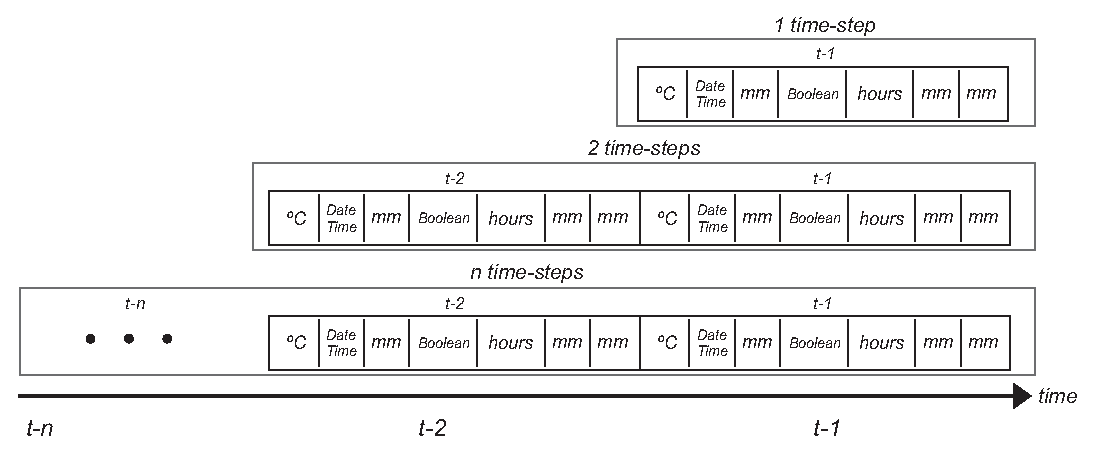
\includegraphics[scale=0.7]{capitulo_2/time_steps}
 \caption{Diagram of the time-steps concept }
 \label{img:figure3}
\end{figure}

\newpage

ANNs training become more efficient if certain preprocessing steps are made on data. Normalisation is crucial to prepare data to made it suitable for training, without this step training would be slow and ineffective. In order to minimize bias into each input feature that have widely different scales, this process is made to scale down data into a similar range \cite{yaldi2009improving}. There are many types of normalisation procedures such as statistical normalisation, that produces data where each feature has a zero mean and a unit variance and Min-Max normalisation that rescales features from one range to a new one depending on the type of activation function    

To keep data inside the constraints of the tangent sigmoid transfer, fitting it into the $[-1, 1]$ interval and making it proper for training, the dataset was normalised by the Min-Max normalisation method demonstrated by the Eq. \ref{eq:solve19}. Then the algorithm was set to run and train all the ANNs models. It was generated 200 individual rainfall forecasting ANNs based on the described methodology, the results of this research are the accuracy of each individual ANN.

\begin{equation}
 \label{eq:solve19}
 Z_i^p = -((\frac{-2(u_i - x_i^p)}{u_i - l_i}) + 1)
\end{equation}

%%\begin{figure}[htbp]
%\begin{figure}[H]
%\tiny \caption{\small Ilustração do sistema operacional como interface entre o usuário e os recursos do sistema. \label{S.O.}}
%% o que está dentro do colchetes é o que aparecerá na lista de figuras.
%\vspace{-0.3 cm}
%\begin{center}
%\begin{psfrags}
%\epsfxsize=4cm
%\centerline{
\includegraphics[width=4.0 cm]{./capitulo_2/tux-linux.eps}}
%\end{psfrags}
%{\small Fonte: Adaptado de \citeonline{llgarver_sept70}}
%\end{center}
%\end{figure}
%
%\newpage % para passar o exemplo de citação para a próxima página.


%-------------------------------------------------------------------------------------------
%\setlength{\headsep}{1.5cm} % Distância entre a margem superior do quadro do texto e o cabeçalho.
\chapter{RESULTS AND DISCUSSION }
\label{chapter:servidores_linux}
\vspace{-2cm}


Brazil is a country of continental dimensions with contrasting climates, which were represented by the chosen locations. The World Meteorological Organisation (WMO) establishes the general procedures to calculate the monthly 30 year standard normals and averages \cite{wmo1989calculation}, which are important climatological variables that describes the climatic conditions of a given location. This index were used to contradistinguish the high variability of climate conditions that the ANN structures had to handle. The two opposite climate conditions were Campo Mourão and Jaguaruana, the normals of both locations are represented by Fig. \ref{img:figure4}.


\begin{figure}[htbp]
\subfloat[Campo Mourão]{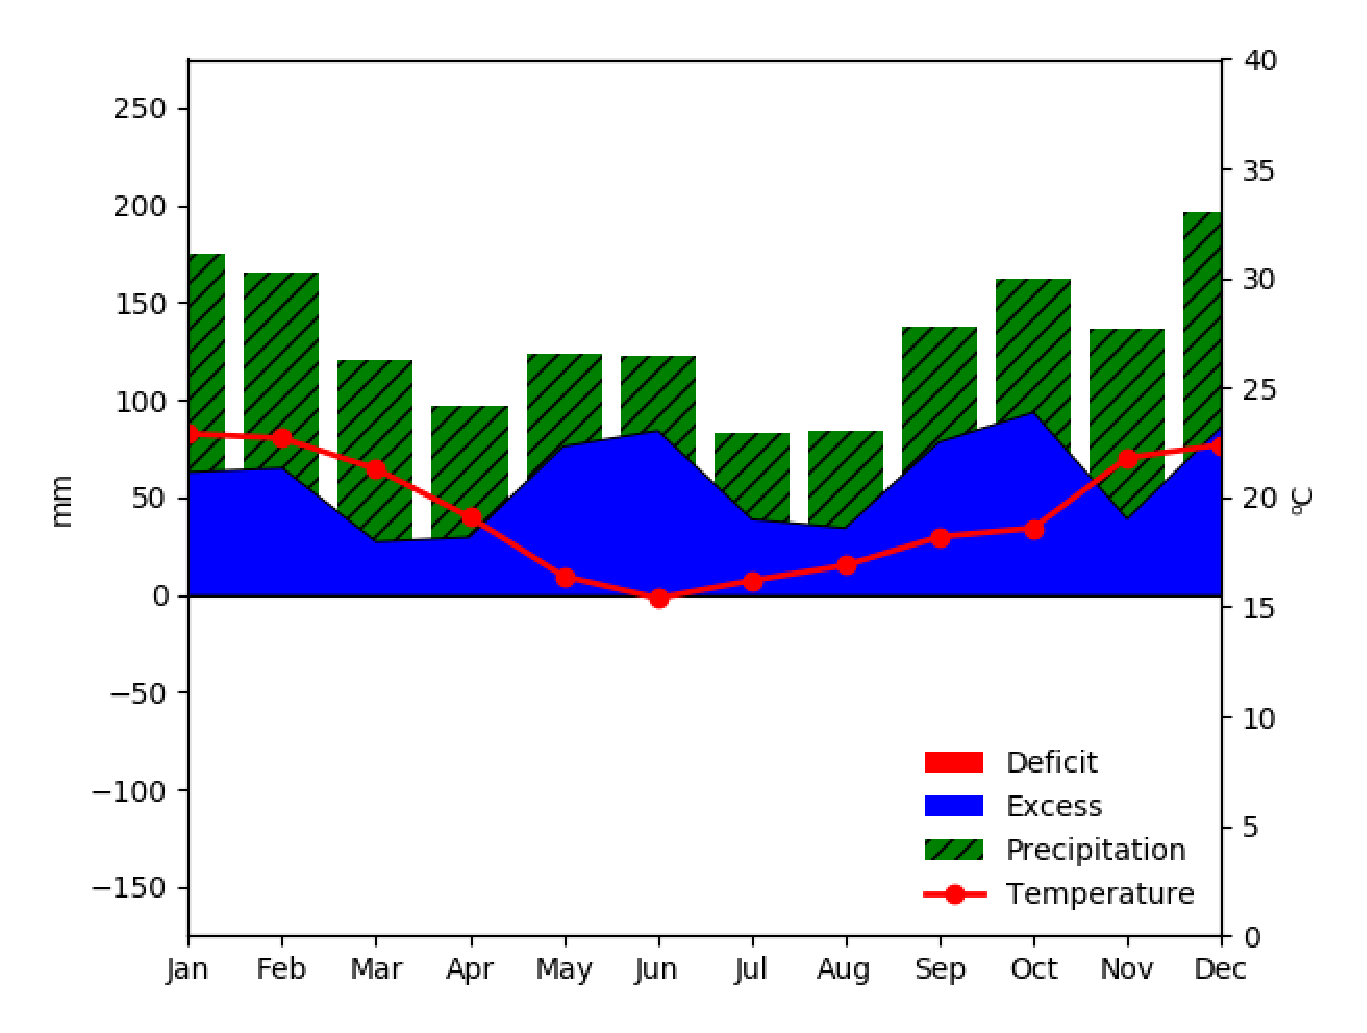
\includegraphics[scale=0.37]{capitulo_3/campo_moral_normal}}
\subfloat[Jaguaruana]{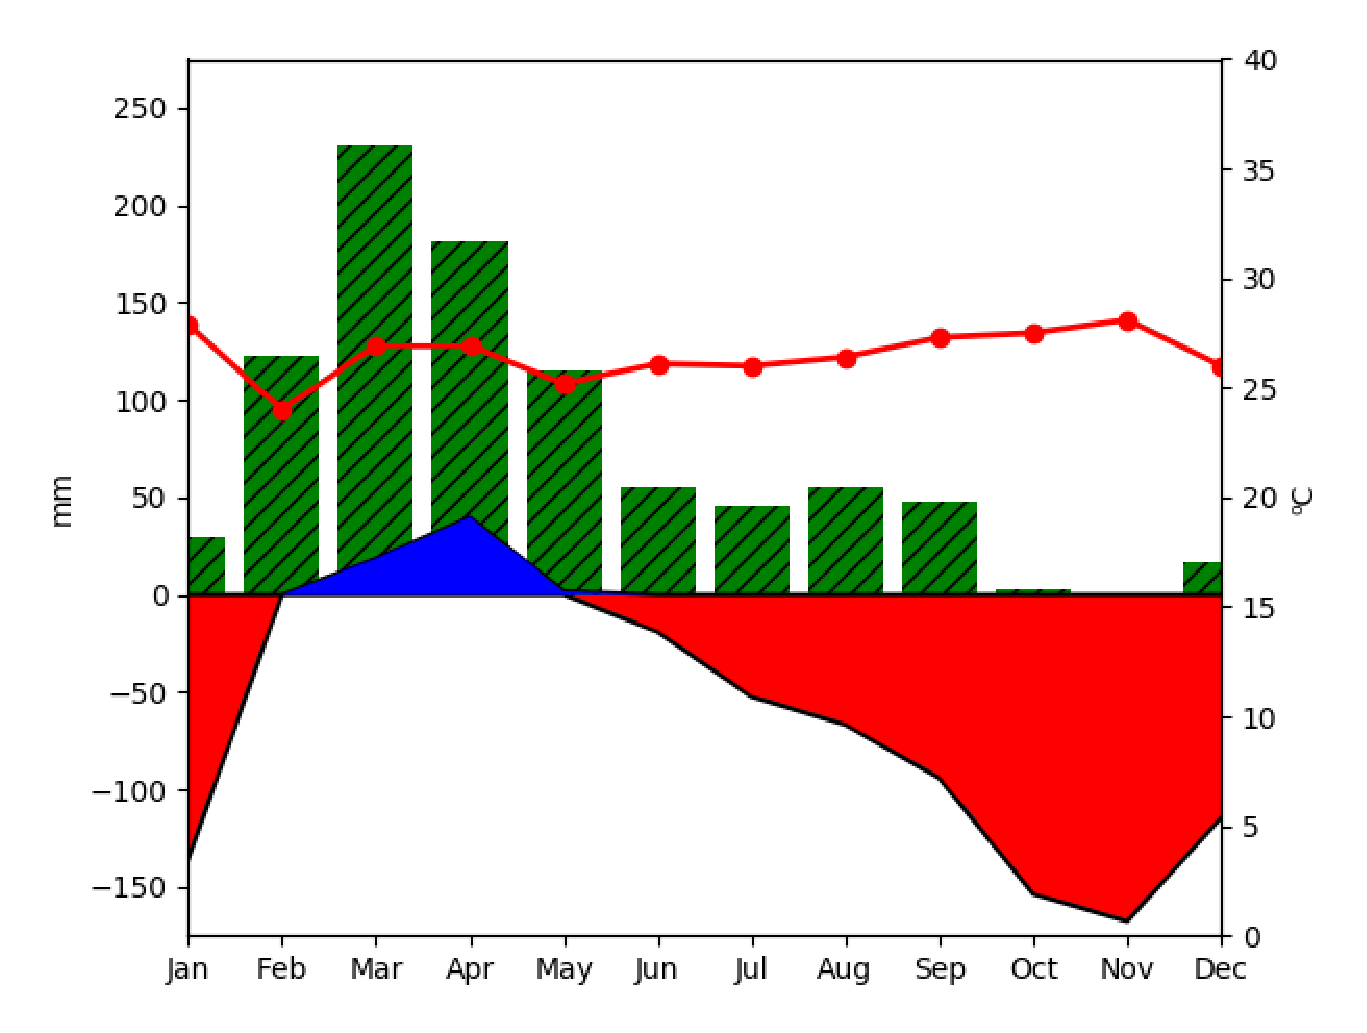
\includegraphics[scale=0.37]{capitulo_3/jaguaruana_normal}}
\caption{Thornthwaite Water Balance and Normal Temperature}
\label{img:figure4}
\end{figure}


Campo Mourão have an subtropical humid mesothermal weather with hot summers and not frequent frosts, the precipitation is well distributed with an accumulated volume of 1603 \textit{mm} there is allegedly no water deficit throughout the year, in contrast Jaguaruana have an tropical savanna climate with water deficit across the year with exception of the months from February to May with an accumulated precipitation of 906 \textit{mm}, the location is an  good representation of the Brazilian semi-arid region. Between these two contrasting climates there are the climes of all the other locations used in this paper, the climate of each location lays among the Jaguaruana tropical savanna and the Campo Mourão humid mesothermal weather. Given the conditions if it were used only one ANN structure for all locations and seasons the noise would be high, and both the accuracy and precision would decay. 

To summarise all the the ANNs assertiveness or the capacity to retrieve information in an general perspective, it was computed the mean accuracy percentage average for all locations for each time range ($[3,...,7]$\textit{days}) and season. In the Fig. \ref{img:figure5} it is shown the summarisation both for the \textit{autoassociative} (a) and \textit{heteroassociative}(b) capabilities of the ANNs structures, the auto-association is the phenomenon of associating the input vector with itself as the output as called by estimation capacity, and the hetero-association is that of recalling a related vector given an input vector or the forecasting capacity \cite{rao1995c++}. 


\begin{figure}[htb!]
 \centering
 \subfloat[autoassociative]{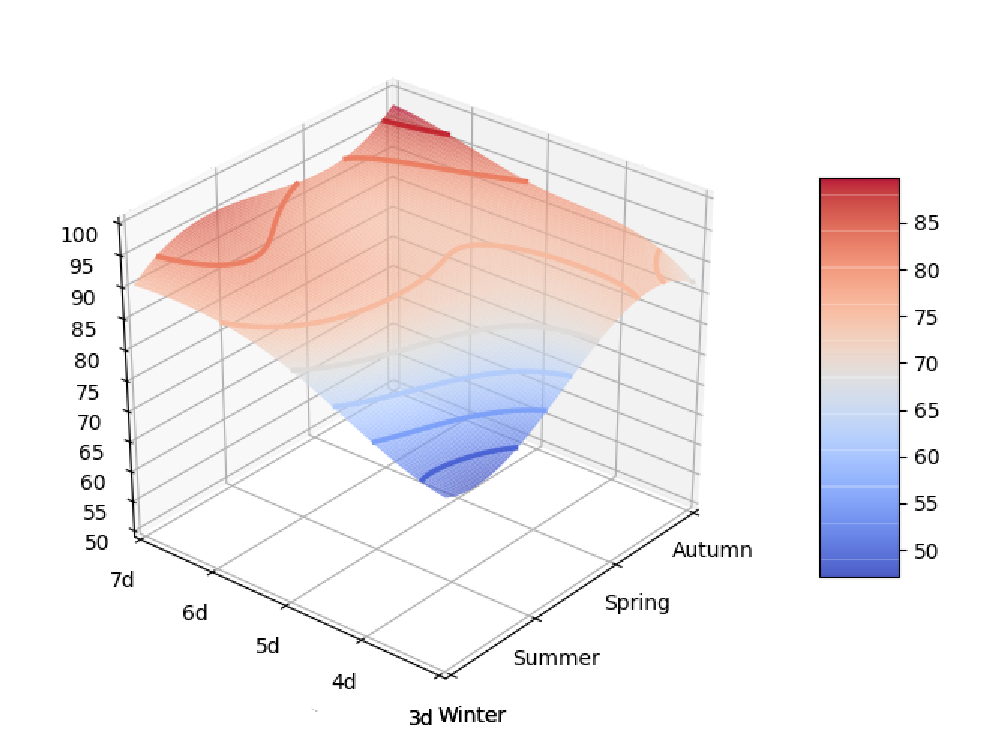
\includegraphics[scale=0.5]{capitulo_3/estimate_accuracy_2}}
 \subfloat[heteroassociative]{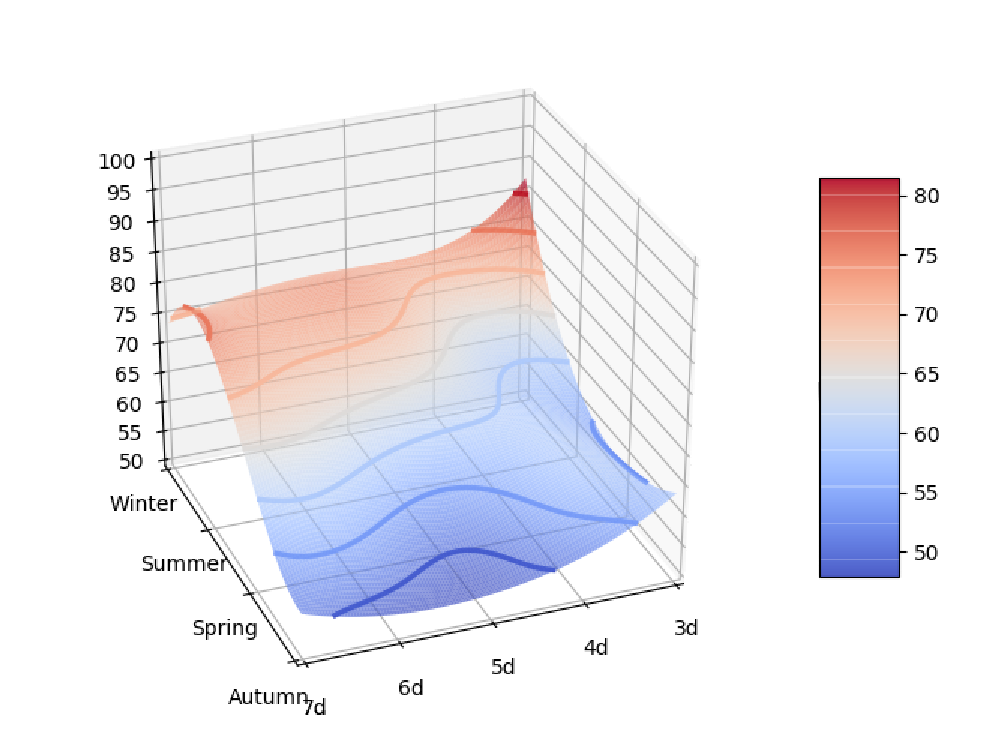
\includegraphics[scale=0.5]{capitulo_3/forecasting_accuracy2}}
 \caption{Summary of ANNs autoassociative (a) and heteroassociative(b) performance}
  \label{img:figure5}
\end{figure}


When trying to self associate, the less accurate ANN was the one trained with winter data for a cumulative period of three days and had an accuracy of 77.15\% for all regions, 
The most accurate were trained with autumn data and an period of seven days achieving a accuracy of 97.61\% , between all ANNs and cumulative periods the estimation performance average was of 89.18\% indicating that the ANN was able to recall the input variables and associate it with the desired output, which is an quality indicative of the chosen inputs variables.

Different from estimation, the forecasting performance had an increased performance variance, in its least accurate point which were in autumn with an accumulated period of 6 days, the ANN structure had an accuracy of 53.14\%, when most accurate it had an forecasting success of 87.14\% and were in winter with an 3 accumulated days. The Artificial Neural Networks that had the best performance were the ones that had their weights adjusted with data from winter and summer.  Relatively to other studies the performance was acceptable, \citeauthor{valipour2016optimization}  \citeyear{valipour2016optimization} while detecting drought and wet years obtained an average correlation of 0.90, in the prediction stage the model was mostly accurate and dependant on the levels of deforestation. \citeauthor{rivero2015short} \citeyear{rivero2015short} developed a methodology based on ANNs to forecast rainfall on a monthly period with incomplete datasets, the author utilised the symmetric mean absolute percentage error (SMAPE) as a performance metric, the best performing model had an score of 0.51 which the author classifies as almost acceptable.

In Brazil on latitudes near the equator line like the city of Jaguaruana, winter is the time of year that the rainfall index is usually higher. In summer this index tend to fall, however at lower latitudes this indices reverse and winter happens to be the dry season of the year, in both situations the climate is well defined making it easier for the neural network to generalize its knowledge and accurately forecast the rainfall occurrence, winter in all the accumulated periods was the most predictable season.
  
Autumn and spring are transitional epochs and there is a mix of climate characteristics both from winter to summer, as from summer to winter. In these seasons the artificial neural networks notably had greater difficulty in forecasting clearly whether or not there would be rainfall, autumn was the least predictable season. 
Despite the forecast accuracy being smaller in both seasons this is an important result, it indicates that it was wise to create an model for each climate season, if this were not done and the general model have been divided into only 2 times of the year, this effect would have been diluted in the results vector, so that the shape of the forecast chart in Fig \ref{img:figure5} would become flattened. 

In the first half of the year of southern hemisphere are contained the summer and fall, the inability of the network to generalise its knowledge of autumn would have negatively impacted the summer forecast capacity, in the second half of the year the effect would have been the same with the difference that the forecasting ability of winter would be impacted by the spring. In the Fig. \ref{img:figure6} is shown the detailed performance of each ANN with an colour scale that visually represents the relative accuracy of the model, by this figure is clear the predominance of the ANNs models being more accurate both on summer and winter, the combination of location and season with the most notable performance was Maceio on winter and the worst was Campo Mourão on autumn.  

\begin{figure}[htb!]
 \centering
  \caption{ANNs accuracy percentage performance}
 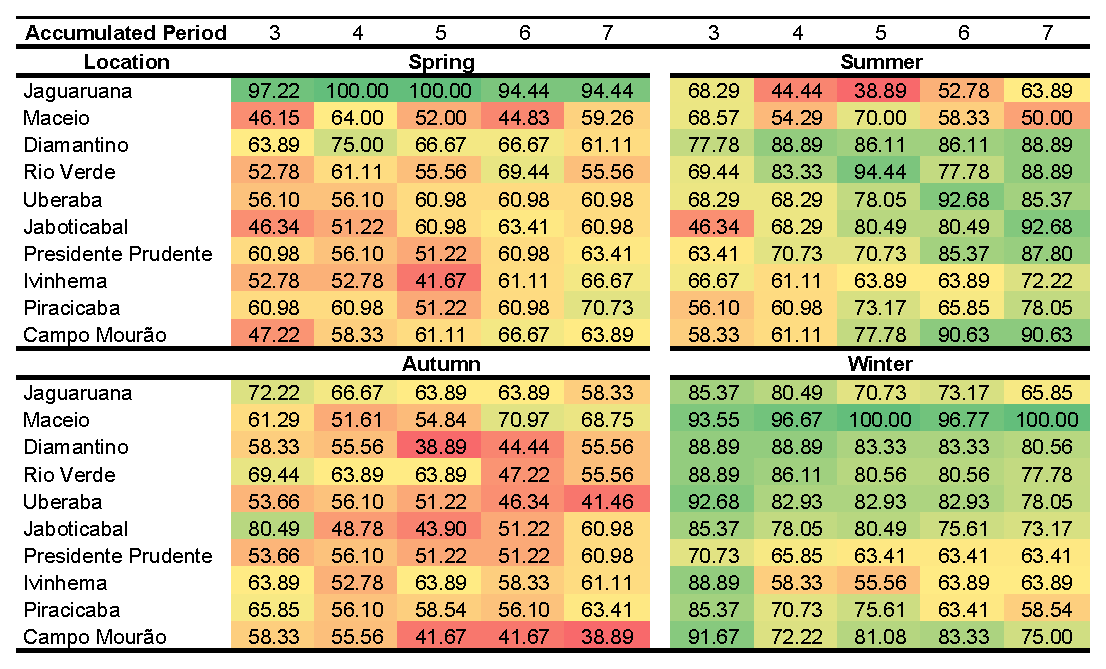
\includegraphics[scale=0.9]{capitulo_3/general_table}
 \label{img:figure6}
\end{figure}

When oceanic air masses moves to continent inland they loose water through precipitation and the remaining of this masses become progressively depleted in water vapour, this phenomena can be called continentality effect. By reaching orographic obstacles, the condensation and rainfall associated with the adiabatic cooling of these raising air masses and further deplete the vapor of it, which is called altitude effect \cite{vuille2003modeling}. The continentality and altitude effect therefore can be important as sources of rainfall variability over the years and as shown by Fig.\ref{img:figure7} and Fig. \ref{img:figure8} impact on the ANNs prediction performance. 


\begin{figure}[htb!]
 \centering
  \caption{The effect of continentality on the ANNs accuracy at all seasons.}
 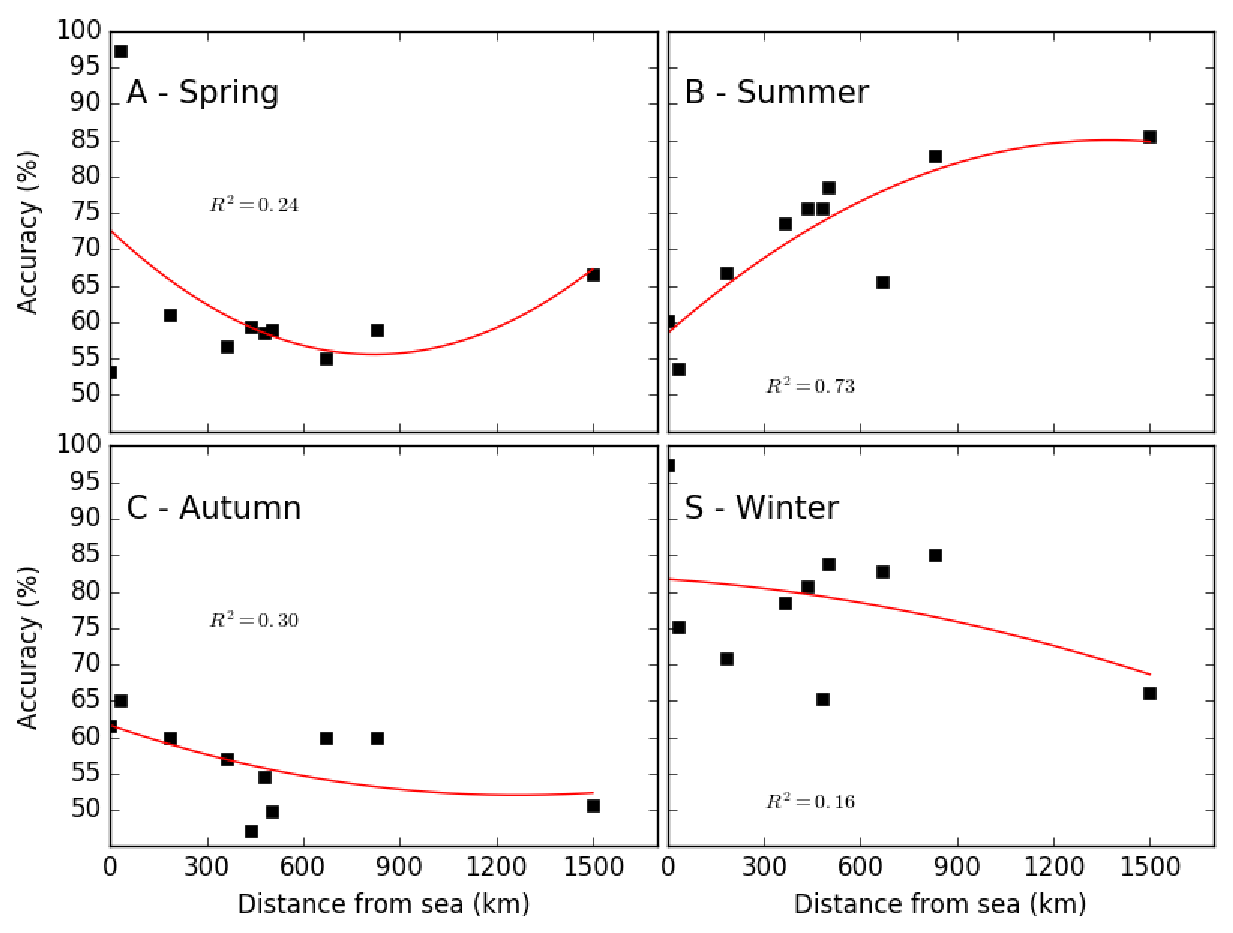
\includegraphics[scale=0.78]{capitulo_3/continentality_effect}
 \label{img:figure7}
\end{figure}
\begin{figure}[htb!]
 \centering
  \caption{The effect of altitude on the ANNs accuracy at all seasons.}
 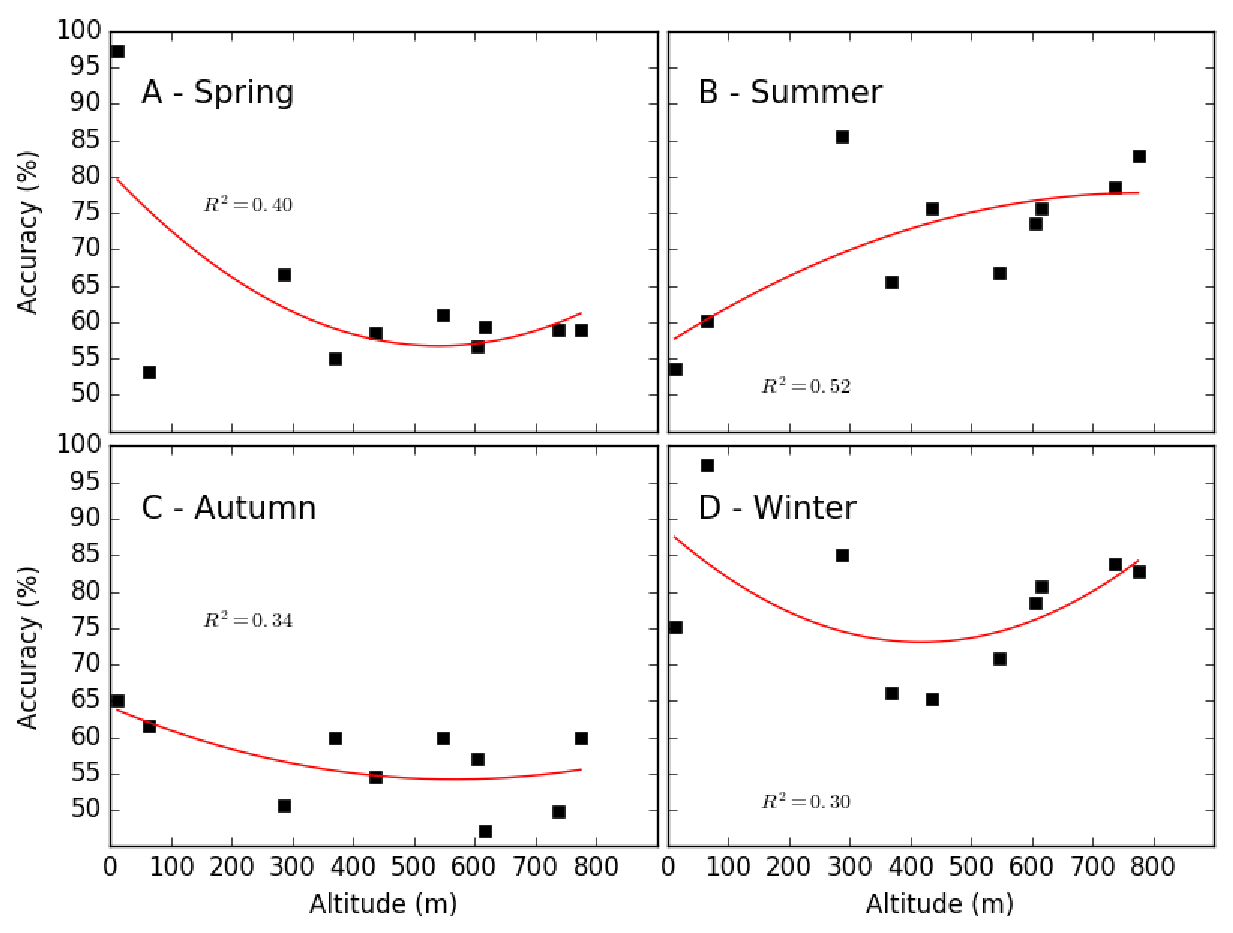
\includegraphics[scale=0.78]{capitulo_3/topographic_effect}
 \label{img:figure8}
\end{figure}

\newpage
The Continentality effect was a more prominent source of noise to the ANNs at summer, the closer to the sea the bigger it was the impact on the ANNs accuracy which is actually coherent. Summer is the season that the amount of solar radiation and energy in the atmosphere are higher and consequently the amount of oceanic air masses coming inward are greater. These air masses are highly unstable closer to the sea and tend to loose its strength and stabilise as they move into the continent, the impact of this phenomena on the ANNs forecasting accuracy is represented in the Fig. \ref{img:figure7} graph B.

On winter the effect of continentality on the ANNs is quite the opposite of what happens on summer, mainly because the amount of maritime air masses is lower than summer which reduces the climatic variability and reverses accuracy tendency of the ANNs as shown in the graph D of Fig. \ref{img:figure7}. As spring and autumn are transitional seasons the effect of continentality is not quite well defined, on the first half of spring the oceanic air masses behaves more like the ones of winter and on the second half it starts to behaves as the masses of summer, inverting this behaviour on autumn, the effect of continentality on this seasons are shown on graphs A and C of Fig. \ref{img:figure7}. Alvares et al. \cite{alvares2013modeling} described an strong correlation of temperature and the effect of continentality during summer and the opposite on winter which corroborate with the result obtained. 

The Altitude effect on summer behaves closely as the effect of continentality, there is a large amount of steam loaded air masses coming from sea and an increased amount of orographic rainfalls \cite{salati1979recycling} which is apparently a type of precipitation that the ANNs were able of correctly predict as shown by graph B of Fig \ref{img:figure8}. The altitude effect is not as prominent on the accuracy of the ANNs on winter (Fig.\ref{img:figure9} graph D) of which the amount of orographic rainfalls is quite reduced in comparison of summer, and both on spring and autumn it behaves as the continentality effect and by the same reasons. Other studies \cite{gonfiantini2001altitude} on tropical rains described an seasonal variation on rainfall volumes duo to altitude effect being more positive on summer with respects to winter. This seasoned influence is explained duo to the lowering of temperatures and consequent increase of the condensation rate of atmospheric vapour and a greater availability of air moisture on summer when compared to winter .

\begin{figure}[htb!]
 \centering
  \caption{The effect of precipitation volumes on ANN models}
 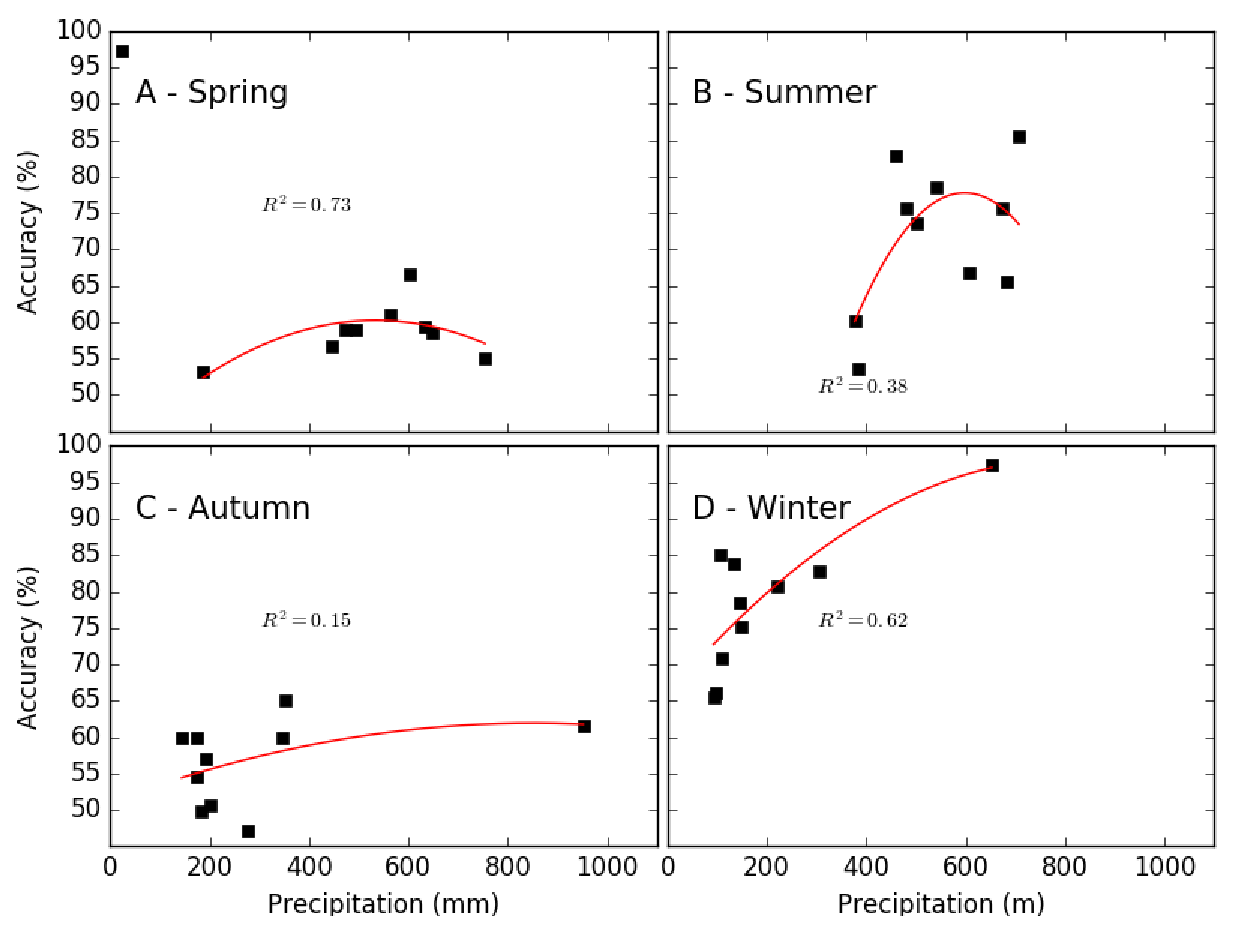
\includegraphics[scale=0.78]{capitulo_3/precipitation_accuracy}
 \label{img:figure9}
\end{figure}

One factor that can affect directly the ANNs accuracy is the rainfall frequency and volume by itself of which lack of exposure to a significant number of rainfall events can make the ANN underforecast and miss its occurrence \cite{kuligowski1998experiments}. As show by Fig. \ref{img:figure9} graphs B and D, on winter and summer the ANNs forecasting accuracy is correlated with the amount of rainfall in the period of which the accuracy of the model increases with the precipitation amount. In spring and autumn the precipitation volume do not affect the accuracy of the model. 

Comparing the results of this paper with previous studies \cite{kumarasiri2006rainfall, kuligowski1998experiments, nasseri2008optimized, hall1999precipitation, ramirez2006linear, rajurkar2002artificial} was difficult firstly because of the disparity of ranges of these studies, some have used short forecasting periods on the scale of hours and others used a monthly scale, secondly these studies were focused on predicting not only the rainfall event but also the precipitation volume, which wasn't the goal of this research. 

















%-------------------------------------------------------------------------------------------
\chapter{CONCLUSION}
\label{cap:cap4}
\vspace{-2cm}

The objective of this paper was to develop an automatic ANN modelling strategy that through the analysis of time series predicts the occurrence of rainfall greater than 5mm for each climatic season for accumulated periods from 3 to 7 days. The study has led to the conclusion that the ANNs can forecast these events with an average accuracy for all the accumulated periods of 78\%  on summer,  71\% on winter, 62\% on spring  and 56\% on autumn. Despite the results, the performance of these models could be improved in future studies, by using training algorithms that are capable of converging on results closer to the global optimum such as training feedforward ANNs with genetic algorithms.

Macroclimatic and mesoclimatic effects, such as the effect of continentality and the effect of altitude as well as the normal precipitation volume, has an direct impact on the forecasting accuracy of the ANNs in well defined seasons. Furthermore despite the relatively lower forecasting performance of transitional seasons, the most important seasons for Brazilian crop production are the summer and winter that are those that the model had best accuracy, nevertheless the results of autumn and spring are still applicable with some limitations. To improve this technic different classificatory algorithms could be implemented, in addition exploratory multivariate statistical procedures, such as principal component analysis or correspondence analysis, would better select input variables. However this type of ANNs structures are suited as an indicative of rainfall eminence and in future studies separate models can be developed to forecast its volume.

%-------------------------------------------------------------------------------------------
%\chapter{RESULTADOS E DISCUSSÕES}
\label{cap:cap5}
\vspace{-2cm}

Neste capítulo será apresentado os resultados...


\newpage  % (retirar este comando depois de escrever o capítulo)

%%-------------------------------------------------------------------------------------------
%\chapter{CONCLUSÕES}
\label{cap:cap6}
\vspace{-2cm}

Conclui-se que...

\newpage    % (retirar este comando depois de escrever o capítulo)

%%------------------------------------------------------------------------------------------
%
%\citeoption{abnt-title-command=yes}
%
%\newcommand{\bibtextitlecommand}[2]{\textbf{#2}}         % Este comando coloca os títulos dos trabalhos em negrito
\renewcommand{\bibname}{\hspace{1.3cm}REFERÊNCIAS~~~~~~~~~~~~}     % Este comando renomeia o nome da seção bibliográfica

%%-------------------------------------------------------------------------------------------
%\bibliographystyle{abnt-alf}                             % Estilo ABNT para referências no modo AUTOR-DATA

%----------Me dá o controle sobre o capítulo de referências------------------------------
\makeatletter
\def\@makechapterhead#1{%
  \vspace*{-40\p@}%
  {\parindent \z@ \raggedright \normalfont
    \ifnum \c@secnumdepth >\m@ne
        \normalsize\bfseries \@chapapp\space \thechapter
        \par\nobreak
        \vskip 20\p@
    \fi
    \interlinepenalty\@M
    \normalsize \bfseries #1\par\nobreak
    \vskip 12\p@
  }}
\def\@makeschapterhead#1{%
  \vspace*{40\p@}%
  {\parindent \z@ \raggedright
    \normalfont
    \interlinepenalty\@M
    \normalsize \centering \bfseries  #1\par\nobreak
    \vskip 25\p@
  }}
\makeatother
%-------------------------------------------------------------------------------------------

\bibliography{./bibliografia/bibliografia1}              % Arquivo .bib com as referências
%\begin{spacing}{0.0}    % Serve para controlar a margem superior da folha de referências.
%\end{spacing}
%-------------------------------------------------------------------------------------------

\appendix
\renewcommand{\ABNTtravessao}{-}
\setlength{\ABNTanapindent}{0cm}
\renewcommand{\ABNTaposindicativoanap}
{\protect\centering\protect}

%\renewcommand{\appendixname}{\hspace{1.3cm}APÊNDICE}
%\chapter{LINUX}
\label{apa:linux}
\vspace{-2cm}

Neste capítulo será abordado o surgimento e a evolução do sistema operacional Linux. \cite{garver_sept70}.

\section*{\hspace{1.3cm}APÊNDICE A.1 - HISTÓRICO DO LINUX}
\label{secapa:linux}
Atualmente, ... 

Segundo \citeonline{machado}, o sistema operacional (SO), possui inúmeras funções, as quais podem ser resumidas em duas:
\begin{itemize}
\item \textbf{Facilidade de acesso aos recursos:} consiste em ser totalmente transparente ao usuário a maneira como funciona um computador \index{computador} paralelo \index{computador!paralelo} , ou seja, para um usuário não importa como um arquivo que está em um disquete será lido, mas sim que o mesmo será lido, resumindo, um usuário \index{usuário} não precisa saber como será realizado essa ação e suas inúmeras etapas;
\end{itemize}

%\begin{figure}[htbp]
%\begin{figure}[H]
%\tiny \caption[Ilustração é um exemplo de figura]{\small Ilustração.} % o que está dentro dos colchetes é o que vai aparecer na lista de figuras. Tenha essa possibilidade a mais, veja que a figura do capítulo 2 está diferente.
%\vspace{-0.3 cm}
%\begin{center}
%\begin{psfrags}
%\epsfxsize=4cm
%\centerline{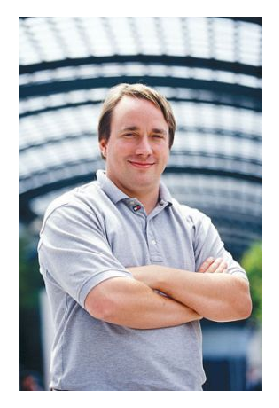
\includegraphics[width=4.0 cm]{./apa/linus_torvalds.eps}}
%\end{psfrags}
%{\small Fonte: Adaptado de \citeonline{machado}}
%\end{center}
%\label{torvalds}
%\end{figure}
%

%
%\chapter{AINDA FALANDO DO LINUX}
\label{apb:linux}
\vspace{-2cm}

Neste capítulo será abordado o surgimento e a evolução do sistema operacional Linux.

\section*{\hspace{1.3cm}APÊNDICE B.1 - MELHORIAS PARA O LINUX EM UM AMBIENTE COORPORATIVOS DE DUAS GRNDES FRNTES INTERPRETATIVAS}
\sectionmark{\protect\parbox{.9\textwidth}{APÊNDICE B.1 - MELHORIAS PARA O LINUX EM UM AMBIENTE COORPORATIVOS DE DUAS GRNDES FRNTES INTERPRETATIVAS}}
\label{secapb:linux}
Atualmente, ... 

\begin{itemize}
\item \textbf{Facilidade de acesso aos recursos:} consiste em ser totalmente transparente ao usuário a maneira como funciona um computador, ou seja, para um usuário comum \index{usuário!comum} não importa como um arquivo que está em um disquete será lido, mas sim que o mesmo será lido, resumindo, um usuário \index{usuário} não precisa saber como será realizado essa ação e suas inúmeras etapas. \cite{machado};
\end{itemize}

%%\begin{figure}[htbp]
%\begin{figure}[H]
%\tiny \caption{\small Novo sistema operacional.}
%\vspace{-0.3 cm}
%\begin{center}
%\begin{psfrags}
%\epsfxsize=4cm
%\centerline{
\includegraphics[width=4.0 cm]{./apb/gnu-linux.eps}}
%\end{psfrags}
%{\small Fonte: \citeonline{machado}}
%\end{center}
%\end{figure}

Para facilitar a vida dos usuários, um exemplo de tabela longa.

\begin{centering}
\footnotesize
\begin{longtable}{c|c|c|c|c|c|c|c|c|c|c}
\captionsetup{width=14.8cm}
\caption{\label{tab:5solIEEE}Espaço ~~de ~busca ~combinatório ~reduzido ~($EBCR$) ~de 10, 5, 3 e 2 ~soluções com \textit{gap} de 5\% Para IEEE}\\
\hline
\multirow{3}{*}{Ramos} & \multicolumn{10}{c}{Número Máximo de linhas}\tabularnewline
\cline{2-11} 
 & \multicolumn{2}{c|}{poolreplace=0} & \multicolumn{4}{c|}{poolreplace=1} & \multicolumn{4}{c}{poolreplace=2}\tabularnewline
\cline{2-11} 
 & 5 sol. & 2 sol. & 10 sol. & 5 sol. & 3 sol. & 2 sol. & 10 sol. & 5 sol. & 3 sol. & 2 sol.\tabularnewline
\hline 
\hline
\endfirsthead
\caption[]{(Continuação da tabela da página anterior)}\\
\hline
\multirow{3}{*}{Ramos} & \multicolumn{10}{c}{Número Máximo de linhas}\tabularnewline
\cline{2-11} 
 & \multicolumn{2}{c|}{poolreplace=0} & \multicolumn{4}{c|}{poolreplace=1} & \multicolumn{4}{c}{poolreplace=2}\tabularnewline
\cline{2-11} 
 & 5 sol. & 2 sol. & 10 sol. & 5 sol. & 3 sol. & 2 sol. & 10 sol. & 5 sol. & 3 sol. & 2 sol.\tabularnewline
\hline     
\hline
\endhead
\hline
\multicolumn{11}{r}{\emph{continua.}}
	\endfoot
	\multicolumn{11}{r}{\emph{Fim.}}
	\endlastfoot
\hline 
$n_{1-2}$  & 3 & 1 & 3 & 4 & 2 & 1 & 4 & 3 & 2 & 0\tabularnewline
\hline 
$n_{1-3}$  & 0 & 0 & 0 & 0 & 0 & 0 & 0 & 0 & 0 & 0\tabularnewline
\hline 
$n_{1-5}$  & 1 & 1 & 1 & 1 & 1 & 1 & 1 & 1 & 1 & 1\tabularnewline
\hline 
$n_{2-4}$  & 0 & 0 & 0 & 0 & 0 & 0 & 0 & 0 & 0 & 0\tabularnewline
\hline 
$n_{2-6}$  & 0 & 0 & 0 & 0 & 0 & 0 & 0 & 0 & 0 & 0\tabularnewline
\hline 
$n_{3-9}$  & 0 & 0 & 0 & 0 & 0 & 0 & 0 & 0 & 0 & 0\tabularnewline
\hline 
$n_{3-24}$  & 1 & 1 & 1 & 1 & 1 & 1 & 1 & 1 & 1 & 1\tabularnewline
\hline 
$n_{4-9}$  & 0 & 0 & 0 & 0 & 0 & 0 & 0 & 0 & 0 & 0\tabularnewline
\hline 
$n_{5-10}$  & 0 & 0 & 0 & 0 & 0 & 0 & 0 & 0 & 0 & 0\tabularnewline
\hline 
$n_{6-10}$  & 1 & 1 & 1 & 1 & 1 & 1 & 1 & 1 & 1 & 1\tabularnewline
\hline 
$n_{7-8}$  & 3 & 2 & 3 & 2 & 3 & 3 & 2 & 3 & 2 & 3\tabularnewline
\hline 
$n_{8-9}$  & 0 & 0 & 0 & 0 & 0 & 0 & 0 & 0 & 0 & 0\tabularnewline
\hline 
$n_{8-10}$  & 0 & 0 & 0 & 0 & 0 & 0 & 0 & 0 & 0 & 0\tabularnewline
\hline 
$n_{9-11}$  & 0 & 0 & 0 & 0 & 0 & 0 & 0 & 0 & 0 & 0\tabularnewline
\hline 
$n_{9-12}$  & 0 & 0 & 0 & 0 & 0 & 2 & 0 & 0 & 0 & 0\tabularnewline
\hline 
$n_{10-11}$  & 1 & 0 & 1 & 0 & 1 & 1 & 0 & 1 & 0 & 1\tabularnewline
\hline 
$n_{10-12}$  & 1 & 1 & 1 & 1 & 1 & 1 & 1 & 1 & 1 & 1\tabularnewline
\hline 
$n_{11-13}$  & 1 & 1 & 1 & 1 & 1 & 1 & 1 & 1 & 1 & 1\tabularnewline
\hline 
$n_{11-14}$  & 0 & 0 & 0 & 0 & 0 & 1 & 0 & 0 & 0 & 0\tabularnewline
\hline 
$n_{12-13}$  & 0 & 0 & 0 & 0 & 0 & 0 & 0 & 0 & 0 & 0\tabularnewline
\hline 
$n_{12-23}$  & 0 & 0 & 0 & 0 & 0 & 0 & 0 & 0 & 0 & 0\tabularnewline
\hline 
$n_{13-23}$  & 0 & 0 & 0 & 0 & 0 & 0 & 0 & 0 & 0 & 0\tabularnewline
\hline 
$n_{14-16}$  & 1 & 1 & 1 & 1 & 1 & 1 & 1 & 1 & 1 & 1\tabularnewline
\hline 
$n_{15-16}$  & 0 & 0 & 0 & 0 & 0 & 0 & 0 & 0 & 0 & 0\tabularnewline
\hline 
$n_{15-21}$  & 0 & 0 & 0 & 0 & 0 & 0 & 0 & 0 & 0 & 0\tabularnewline
\hline 
$n_{15-24}$  & 0 & 0 & 0 & 0 & 0 & 0 & 0 & 0 & 0 & 0\tabularnewline
\hline 
$n_{16-17}$  & 0 & 0 & 0 & 0 & 0 & 0 & 0 & 0 & 0 & 0\tabularnewline
\hline 
$n_{16-19}$  & 0 & 0 & 0 & 0 & 0 & 0 & 0 & 0 & 0 & 0\tabularnewline
\hline 
$n_{17-18}$  & 0 & 0 & 0 & 0 & 0 & 0 & 0 & 0 & 0 & 0\tabularnewline
\hline 
$n_{17-22}$  & 0 & 0 & 0 & 0 & 0 & 0 & 0 & 0 & 0 & 0\tabularnewline
\hline 
$n_{18-21}$  & 0 & 0 & 0 & 0 & 0 & 0 & 0 & 0 & 0 & 0\tabularnewline
\hline 
$n_{19-20}$  & 0 & 0 & 0 & 0 & 0 & 0 & 0 & 0 & 0 & 0\tabularnewline
\hline 
$n_{20-23}$  & 1 & 1 & 1 & 1 & 1 & 1 & 1 & 1 & 1 & 1\tabularnewline
\hline 
$n_{21-22}$  & 0 & 0 & 0 & 0 & 0 & 0 & 0 & 0 & 0 & 0\tabularnewline
\hline 
$n_{1-8}$  & 0 & 0 & 0 & 0 & 0 & 0 & 0 & 0 & 0 & 0\tabularnewline
\hline 
$n_{2-8}$  & 0 & 0 & 0 & 0 & 0 & 1 & 0 & 0 & 0 & 0\tabularnewline
\hline 
$n_{6-7}$  & 0 & 0 & 0 & 0 & 0 & 2 & 0 & 0 & 0 & 0\tabularnewline
\hline 
$n_{13-14}$  & 0 & 0 & 0 & 0 & 0 & 1 & 0 & 0 & 0 & 0\tabularnewline
\hline 
$n_{14-23}$  & 1 & 0 & 1 & 0 & 1 & 1 & 0 & 1 & 0 & 1\tabularnewline
\hline 
$n_{16-23}$  & 0 & 0 & 0 & 0 & 0 & 0 & 0 & 0 & 0 & 0\tabularnewline
\hline 
$n_{19-23}$  & 0 & 0 & 0 & 0 & 0 & 0 & 0 & 0 & 0 & 0\tabularnewline
\hline 
\hline 
F.O & 220.28 & 220.28 & 220.28 & 220.28 & 220.28 & 220.28 & 220.28 & 220.28 & 220.2 & 220.2\tabularnewline
\hline
\hline
\multicolumn{11}{l}{\small{Fonte: Dados da pesquisa do autor.}}\tabularnewline
\end{longtable}
\par\end{centering}




%----- Indice Remissivo-------------------------------------------------------
\newpage
\renewcommand{\indexname}{\hspace{1.3cm}ÍNDICE REMISSIVO~~~~~~~~~~~~\vspace{-0.3cm}}
\printindex
%\addcontentsline{toc}{chapter}{\textit{Índice Remissivo}}

\end{document}                                           % Fim do Documento

